\documentclass[10pt]{beamer}
\usepackage{amsmath,amssymb,longtable,hhline}
\usepackage{mathrsfs}
\usepackage{xcolor}
\usepackage{hyperref}
\usepackage{multicol}
\usepackage{anyfontsize}
\usepackage{minted}
\RequirePackage{doi}

\usemintedstyle{tango}
\newcommand{\ltprgsize}{\fontsize{5}{5}\selectfont}
%\newcommand{\ltprgsize}{\footnotesize}
\setminted{fontsize=\footnotesize{},mathescape}

\definecolor{mygreen}{rgb}{0,0.6,0}
\definecolor{mygray}{rgb}{0.5,0.5,0.5}
\definecolor{mymauve}{rgb}{0.58,0,0.82}

\hypersetup{
    bookmarks=true,         % show bookmarks bar?
    unicode=true,           % non-Latin characters in Acrobat’s bookmarks
    pdftoolbar=false,        % show Acrobat’s toolbar?
    pdfmenubar=false,        % show Acrobat’s menu?
    pdffitwindow=false,     % window fit to page when opened
    pdfstartview={FitH},    % fits the width of the page to the window
    pdftitle={Construction techniques of Baikal microbiome research information-computational environment},    % title
    pdfauthor={Evgeny Cherkashin, Alexey Shigarov, Vasily Khristyuk},     % author
    pdfsubject={model driven architecture},   % subject of the document
    pdfnewwindow=true,      % links in new PDF window
    colorlinks=true,       % false: boxed links; true: colored links
    linkcolor=red,          % color of internal links (change box color with linkbordercolor)
    citecolor=green,        % color of links to bibliography
    filecolor=magenta,      % color of file links
    urlcolor=blue           % color of external links
}

\usepackage{pifont}

\usetheme{Warsaw}
\usecolortheme{crane}
%\useinnertheme{rectangles}
%\setbeamertemplate{itemize item}{\scriptsize\hbox{\donotcoloroutermaths\ding{113}}}
\definecolor{darkding}{RGB}{200,56,0}
\setbeamertemplate{itemize item}{\scriptsize\hbox{\color{darkding}{\bfseries\ding{113}}}}
\setbeamertemplate{itemize subitem}{\tiny\raise1.5pt\hbox{\donotcoloroutermaths$\blacktriangleright$}}
\setbeamertemplate{itemize subsubitem}{\tiny\raise1.5pt\hbox{\donotcoloroutermaths$\blacktriangleright$}}
\setbeamertemplate{enumerate item}{\insertenumlabel.}
\setbeamertemplate{enumerate subitem}{\insertenumlabel.\insertsubenumlabel}
\setbeamertemplate{enumerate subsubitem}{\insertenumlabel.\insertsubenumlabel.\insertsubsubenumlabel}
\setbeamertemplate{enumerate mini template}{\insertenumlabel}

\beamertemplatenavigationsymbolsempty

\usepackage{iftex,ifxetex}
\ifPDFTeX
  \usepackage[utf8]{inputenc}
  \usepackage[T1]{fontenc}
  \usepackage[russian]{babel}
  \usepackage{lmodern}
  \usefonttheme{serif}
\else
  \ifluatex
    \usepackage{unicode-math}
    \defaultfontfeatures{Ligatures=TeX,Numbers=OldStyle}
    \setmathfont{Latin Modern Math}
    \setsansfont{Linux Biolinum O}
    \setmonofont{Fira Mono}[Scale=MatchLowercase]
    \usefonttheme{professionalfonts}
    % \setmathfont[
    %     Ligatures=TeX,
    %     Scale=MatchLowercase,
    %     math-style=upright,
    %     vargreek-shape=unicode
    %     ]{euler.otf}
  \fi
\fi

%\useoutertheme{split}
%\useinnertheme{rounded}
\setbeamertemplate{background canvas}[vertical shading][bottom=white!80!cyan!20,top=cyan!10]
%\setbeamertemplate{sidebar canvas left}[horizontal shading][left=white!40!black,right=black]

\graphicspath{{pics/}}

\providecommand{\email}[1]{\texttt{#1}}
\usepackage{changepage}
\newcommand{\GB}[1]{\colorbox{green}{#1}}
\newcommand{\BB}[1]{\colorbox{blue}{#1}}
\newcommand{\RB}[1]{\colorbox{red}{#1}}
\newcommand{\btprgsize}{\fontsize{7}{7}\selectfont}

% --------------------------

% \def\cite#1{(#1)}
\def\doitext{DOI:}
\begin{document}

\setbeamertemplate{background canvas}[vertical shading][bottom=white,top=white]
\setbeamercolor{background canvas}{bg=white}


\title{Web-GIS viewer for active faults data represented as a knowledge graph}
\author[E.~Cherkashin, O.~Lunina, L.~Demyanov, A.~Tsygankov]{\bfseries%
  \underline{Evgeny Cherkashin}, Oksana Lunina,  Leonid Demyanov, Alexander Tsygankov}
\institute{\normalsize Matrosov Institute for System Dynamics and Control Theory, \\ SB RAS, Irkutsk, Russia\\
  Institute of the Earth’s Crust, SB RAS, Irkutsk, Russia\\
  Institute of Mathematics and Information Technologies,\\ Irkutsk State University, Irkutsk, Russia\\
  Institute of Information Techniques and Data Analysis,\\ National Research Irkutsk State Technical University, Irkutsk, Russia
  \\[1em]
\email{\href{mailto:eugeneai@icc.ru}{eugeneai@icc.ru}}%
}
\date[2021]{
ITAMS--2021, Irkutsk, Russia
}

% \date{\today}
\maketitle

\begin{frame}
  \frametitle{Problem statement}
  At IWCI-2021 in ``Integration of Geological Data as a Knowledge Graph'' we proposed the following integration requirements for the collected geological data, so the data can be
  \begin{itemize}
  \item easily accessed
  \item of a standardized representation
  \item integrated with the data sources of the similar structure (access way and data representation paradigm) % e.g. DBPedia.org LOD
  \item thus, reuse the existing data sources for the domain modeling
  \item processed within Big Data paradigm
  \item represented as cartographic work (map) dynamically with/without need of GIS software installation
  \end{itemize}
  The requested requirements were to be fulfilled with the present Semantic Web technologies.
\end{frame}

\begin{frame}[fragile]
  \frametitle{Semantic web technologies \& Knowledge graphs}
  Semantic Web (WEB 3.0) is characterized with
  \begin{itemize}
  \item Technological basis, oriented to the web % User applications are always comprises interconnected distributed web-services.
  \item Standardized data formats, storage, and processing
  \item Open principles of data publishing
  % \item Knowledge Graph (KG) construction techniques
  \item Services for data storage and access provision
  \item Generalized and special user interfaces are used for data presentation\vspace{1em}
  \end{itemize}
%\end{frame}

% Knowledge graphs changed the aspects to the knowledge base as being a part of whole totality of knowledge, implying the obeying the global standards and techniques of its acquisition and processing.

%\begin{frame}
%  \frametitle{Knowledge Graphs}
For the Knowledge Graphs (KG), the following is of interest.
 \begin{itemize}
  \item Converged notions \textbf{data} and \textbf{knowledge} as something is \textbf{known}
  \item Contain data, relations, and metadata (vocabularies)
  \item Distinguished \textbf{node filling in} and \textbf{processing} graph triples, \emph{e.g.}, withing SPARQL queries with UPDATEs
  \item Allow \textbf{postpone} the formal definition of a schema
  \item Three types of graph schemata: \textbf{semantic} (aimed at generalization), \textbf{validating} (\textbf{e.g.} semantics, \textbf{completeness} w.r.t. sets of relations), and \textbf{emergent} (infer a set of generalized structures and \textbf{reconstruct} the KG).
  \end{itemize}
\end{frame}

\begin{frame}
  \frametitle{Knowledge graph: Validating semantic example}
  \centering
  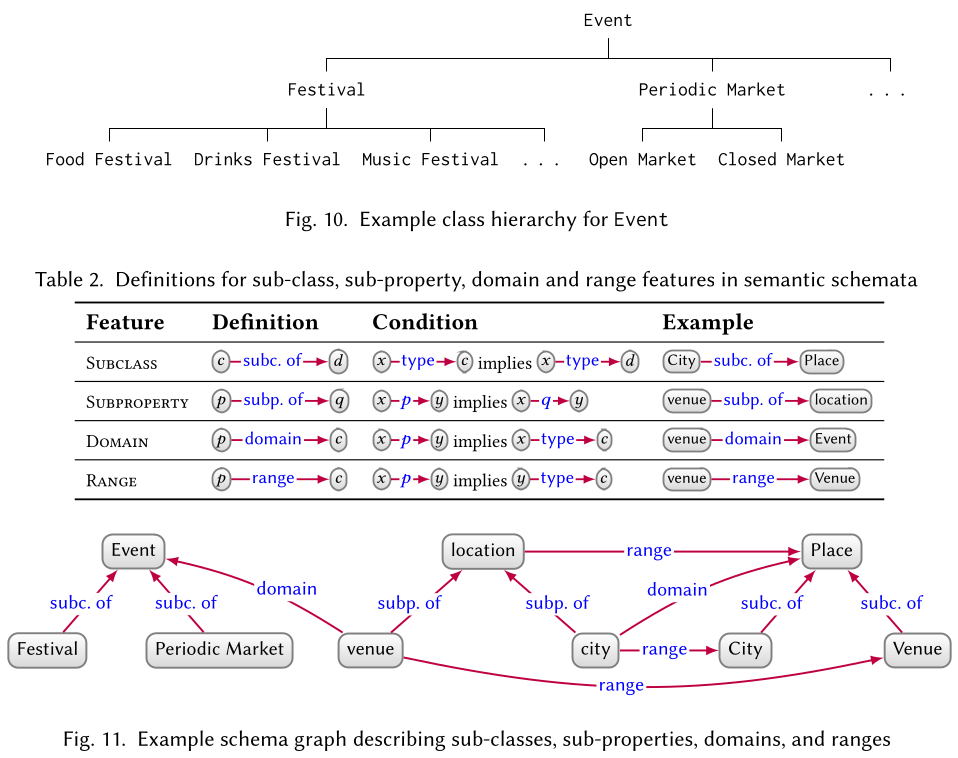
\includegraphics[width=0.9\linewidth]{verify-semantics.png}
\end{frame}


\def\textbfr#1{\textbf{{\color{red}#1*}}}

\begin{frame}
  \frametitle{Linked Open Data (LOD) star evaluation}
  Data are available in
  \begin{itemize}
  \item[\textbfr{1}] any format \textbf{openly}
  \item[\textbfr{2}] a \textbf{structured format}, such as Microsoft Excel file format (.xls)
  \item[\textbfr{3}] a \textbf{non-proprietary structured format}, such as .csv
  \item[\textbfr{4}] \textbf{W3C standards}, like using RDF and employing URIs
  \item[\textbfr{5}] a hypercontent form \textbf{having links to other Linked Open Data sources}
  \end{itemize}
  \begin{flushright}
   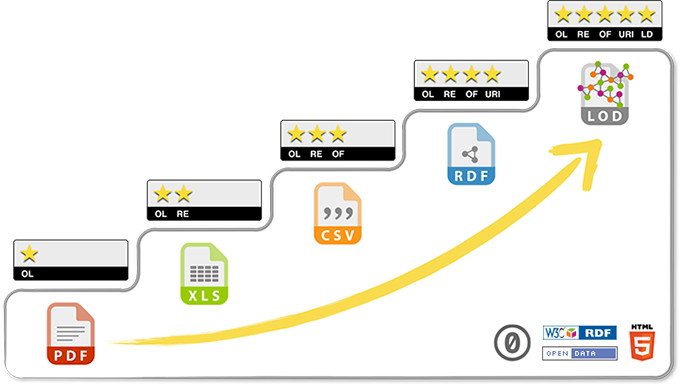
\includegraphics[width=0.7\linewidth]{5-star-lod.png}
  \end{flushright}
\end{frame}

\begin{frame}
  \frametitle{The Aim and the plan}
  The \textbf{aim of the project} is to represent geological data accumulated at IEC SB RAS and other institutes into the Semantic Web infrastructure.

  The \textbf{main problems} to be solved are
  \begin{enumerate}
  \item Design a web-based GIS system, representing data from SPARQL endpoints
  \item Convert the existing data into RDF adhering LOD
  \item Implement natural language query interface using GeoBase (\copyright~Borland${}^{\text{tm}}$) with a conversion into a SPARQL query
  \item Bidirectional versioned data transfer between user GIS (QGIS, OSM Mapnik, Leaflet) and the SW storage % The reason of the usage of OSM Mapmik is the various already implemented data processing service, e.g., GPS traces as raw material for modeling the map.
  \item Implement various analytical functionality for domain problem solving
  \end{enumerate}
\end{frame}

% \begin{frame}
%   \frametitle{}
%   \centering
%   \includegraphics[width=\linewidth]{microbiome-study.png}
% \end{frame}

\begin{frame}
  \centering
  \Large Related works and techniques review
\end{frame}


\begin{frame}
  \frametitle{\textbf{LinkedGeoData} project}
  The project\footnote{Claus Stadler, Jens Lehmann, Konrad Höffner, Sören Auer. LinkedGeoData:
A core for a web of spatial open data. Semantic Web 3 (2012) 333–354. \doi{10.3233/SW-2011-0052}} was to represent OpenSteetMap (OSM) data as a KG,
  \begin{itemize}
  \item Resembles the DBPedia project formalizing Wikipedia data but over the OSM database
  \item Converts SM data into RDF adhering LOD
  \item Designed an ontology for object georeferencing (nodes)
  \item Related the object to DBpedia, GeoNames, icon sets
  \item Developed a taxonomy of the objects on a various levels (Road~\to~Way (list of nodes)) % and Fig 3 of the LGD paper.
  \item Stated the relations between nodes and ways defining complex objects
  \item Implemented REST and SPARQL (does not work now) endpoints for actual data
  \item Had a live updates services from OSM changesets.
  \end{itemize}
\end{frame}


\begin{frame}
  \frametitle{LinkedGeoData project}
  % Figures of Ontology and
  % usage examples
  \centering
  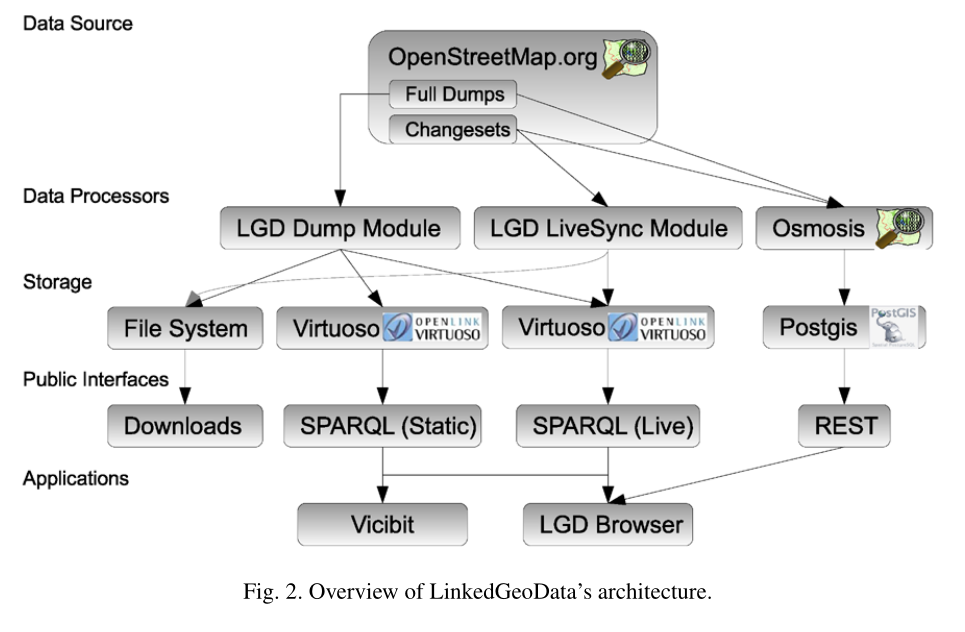
\includegraphics[width=\linewidth]{lgd-sys.png}
\end{frame}

\begin{frame}
  \frametitle{LinkedGeoData project}
  % Figures of Ontology and
  % usage examples
  \centering
  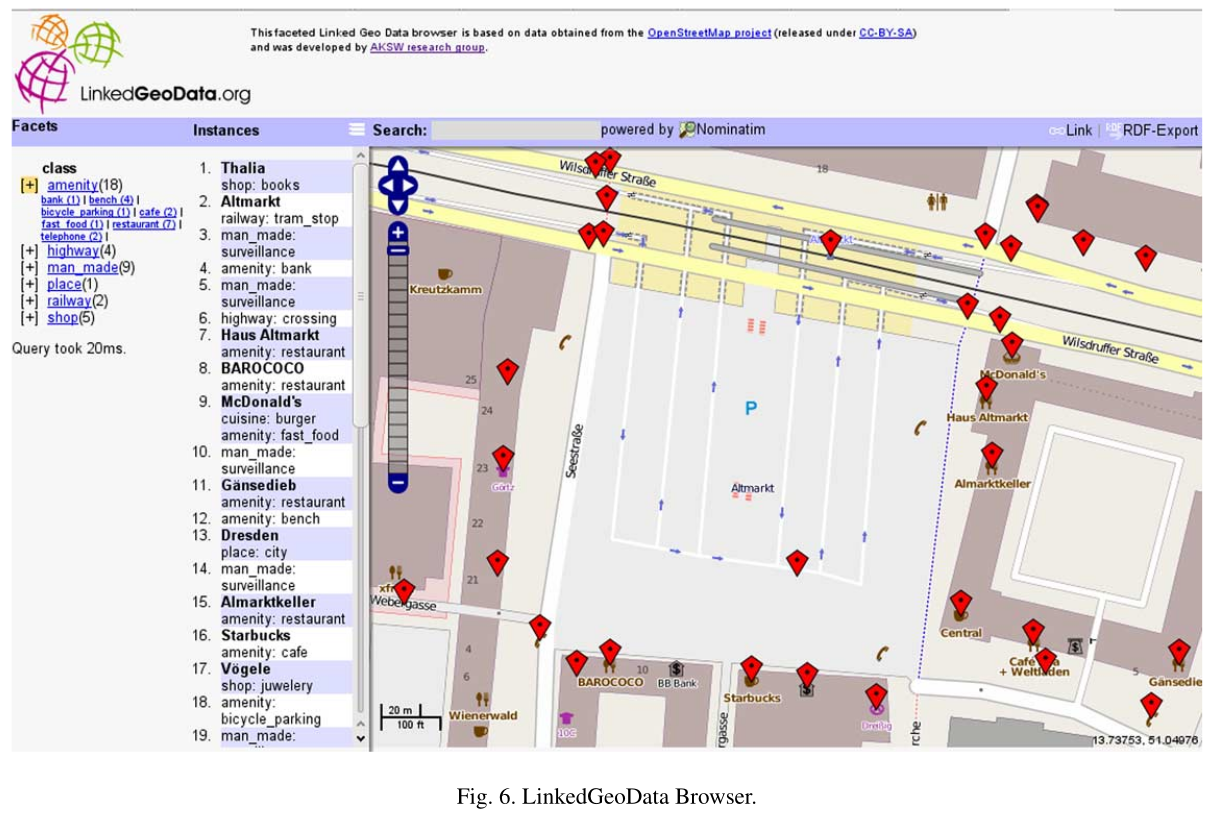
\includegraphics[width=\linewidth]{lgd-screen.png}
\end{frame}


\begin{frame}[fragile]
  \frametitle{\textbf{GeoLink} knowledge graph}
  GeolLink KG\footnote{Michelle Cheatham, Adila Krisnadhi, Reihaneh Amini, Pascal Hitzler, \emph{et al} (2018) The GeoLink knowledge graph, Big Earth Data, 2:2, 131-143, \doi{10.1080/20964471.2018.1469291}}
  \begin{itemize}
  \item Includes diverse information as port calls made by oceanographic cruises, physical sample metadata, research project funding and staffing, and authorship of technical reports
  \item Implements LOD (4 of 5 stars) and federated SPARQL integration
  \item Contains 45 millions RDF triples with ontologies and geo-visualization tools
  \item Describes interlinked \textbf{R2R}, expeditions, \textbf{BCO-DMO}, oceanography, \textbf{IODP}, ocean floor microbiome, \textbf{MBLWHOI}, marine life papers, \textbf{SESAR}, rock samples, \textbf{DataONE}, metadata of external research,  \textbf{AGU-NSF}, projects \& conferences, \textbf{NGDB}, sediment geochemy, \textbf{USAP}, Antarctica ice.
  \end{itemize}
  In the project, an update procedure (harvesting) is implemented to ensure the consistence of the KG w.r.t. the geo-base ontology (GBO).
\end{frame}

\begin{frame}
  \frametitle{GeoLink knowledge graph}
  % Example image from \cite{geolink}
  \begin{center}
  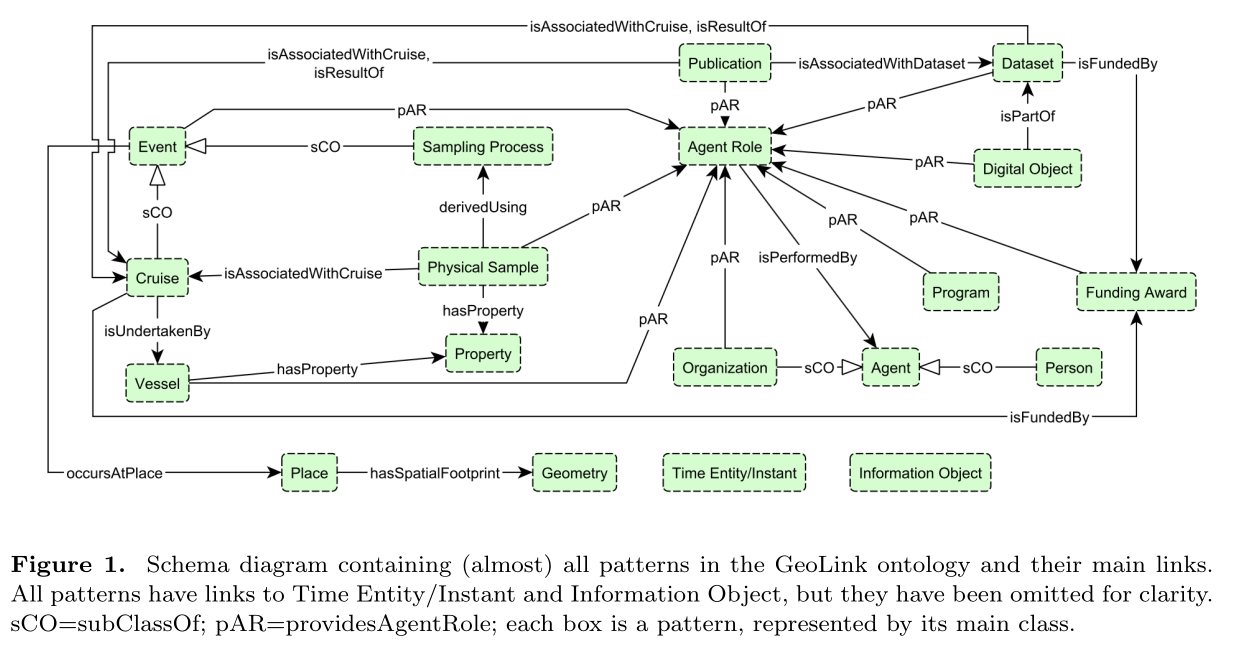
\includegraphics[width=\linewidth]{geolink-onto.png}
  \end{center}
  The GeoLink knowledge graph is deployed at \url{http://data.geolink.org}.
\end{frame}


% The reference \cite{iwaniak} contains a good review of KG GIS activities related to spacial semantic data representation,  importing, crossreferencing and entity relation techniques and tools development.

\begin{frame}
  \frametitle{Integrating LOD into GIS}
  The project\footnote{Tarek Abid, Hafed Zarzour. Integrating Linked Open Data in Geographical
Information System. International Conference on Information Technology for Organization Development. 2014. } deals with developing a web GIS automatically publishing DBPedia data.
  \begin{itemize}
  \item LOD resembles Open Government Data principles
  \item Modules are
    \begin{itemize}
    \item GIS is Google Map API v3
    \item SPARQL used to query DBPedia
    \item Viewing DBPedia data with Data Table plug-in of JQuery
    \end{itemize}
  \item Test application allows user querying celebrities by their home town/city pointed by mouse on the Google Map.
  \end{itemize}
\end{frame}


\begin{frame}
  \frametitle{Integrating LOD into GIS}
  % Figure of GIS and SPARQL query
  \centering
  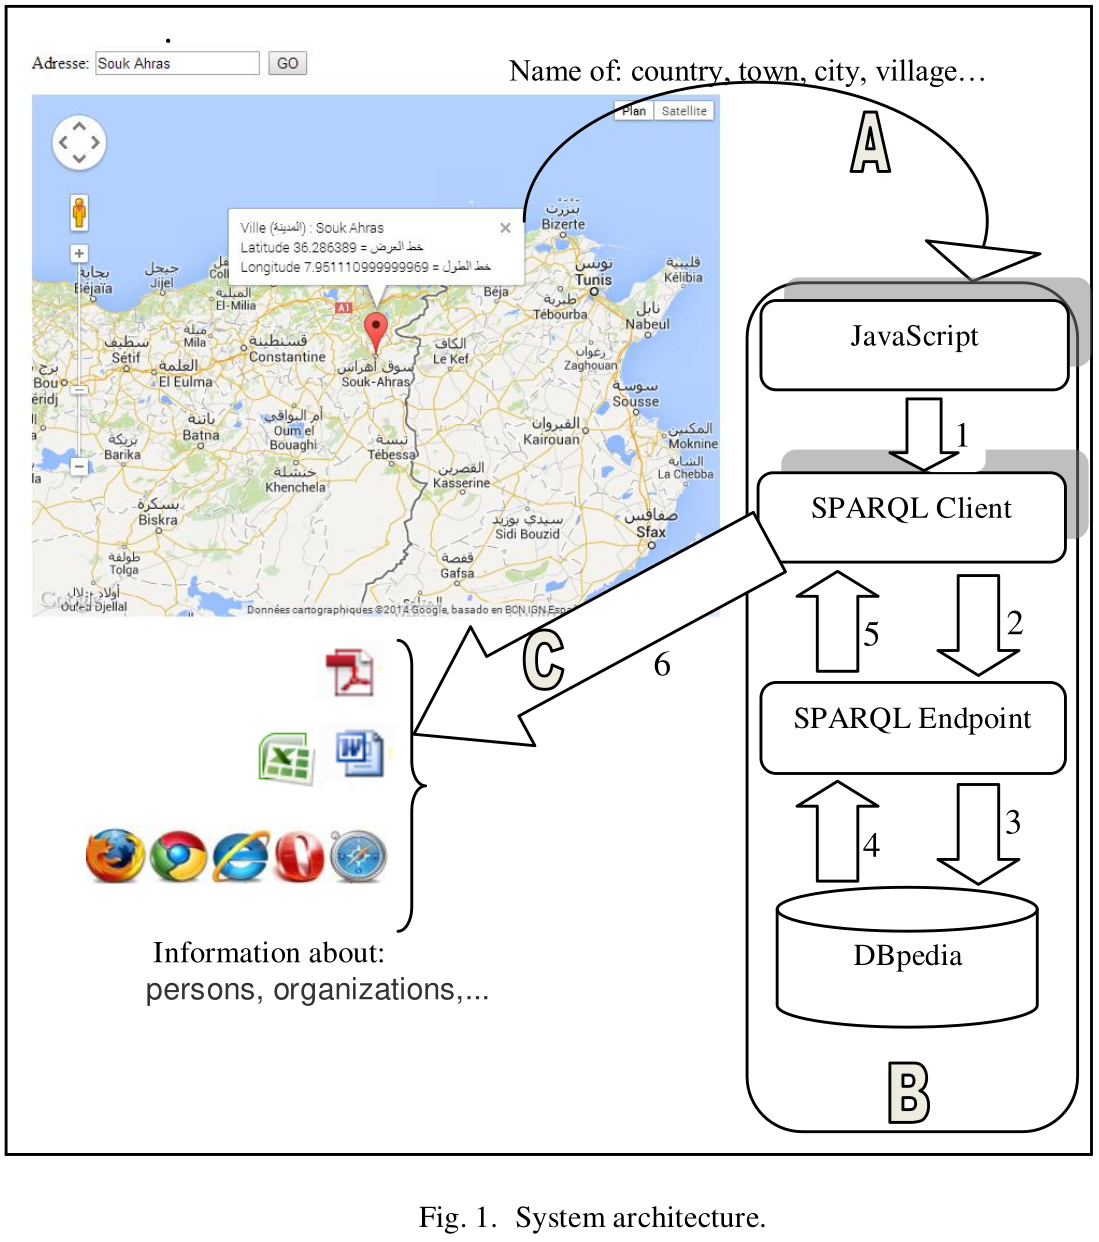
\includegraphics[width=0.65\linewidth]{integrating-lod-gis-arch.png}
\end{frame}

% ----- TODO: Our part ------

\begin{frame}
  \centering
  \Large Results on developing WEB-GIS viewer
\end{frame}


\begin{frame}
  \frametitle{WEB-GIS viewer of active faults of East Siberia}
  \centering
  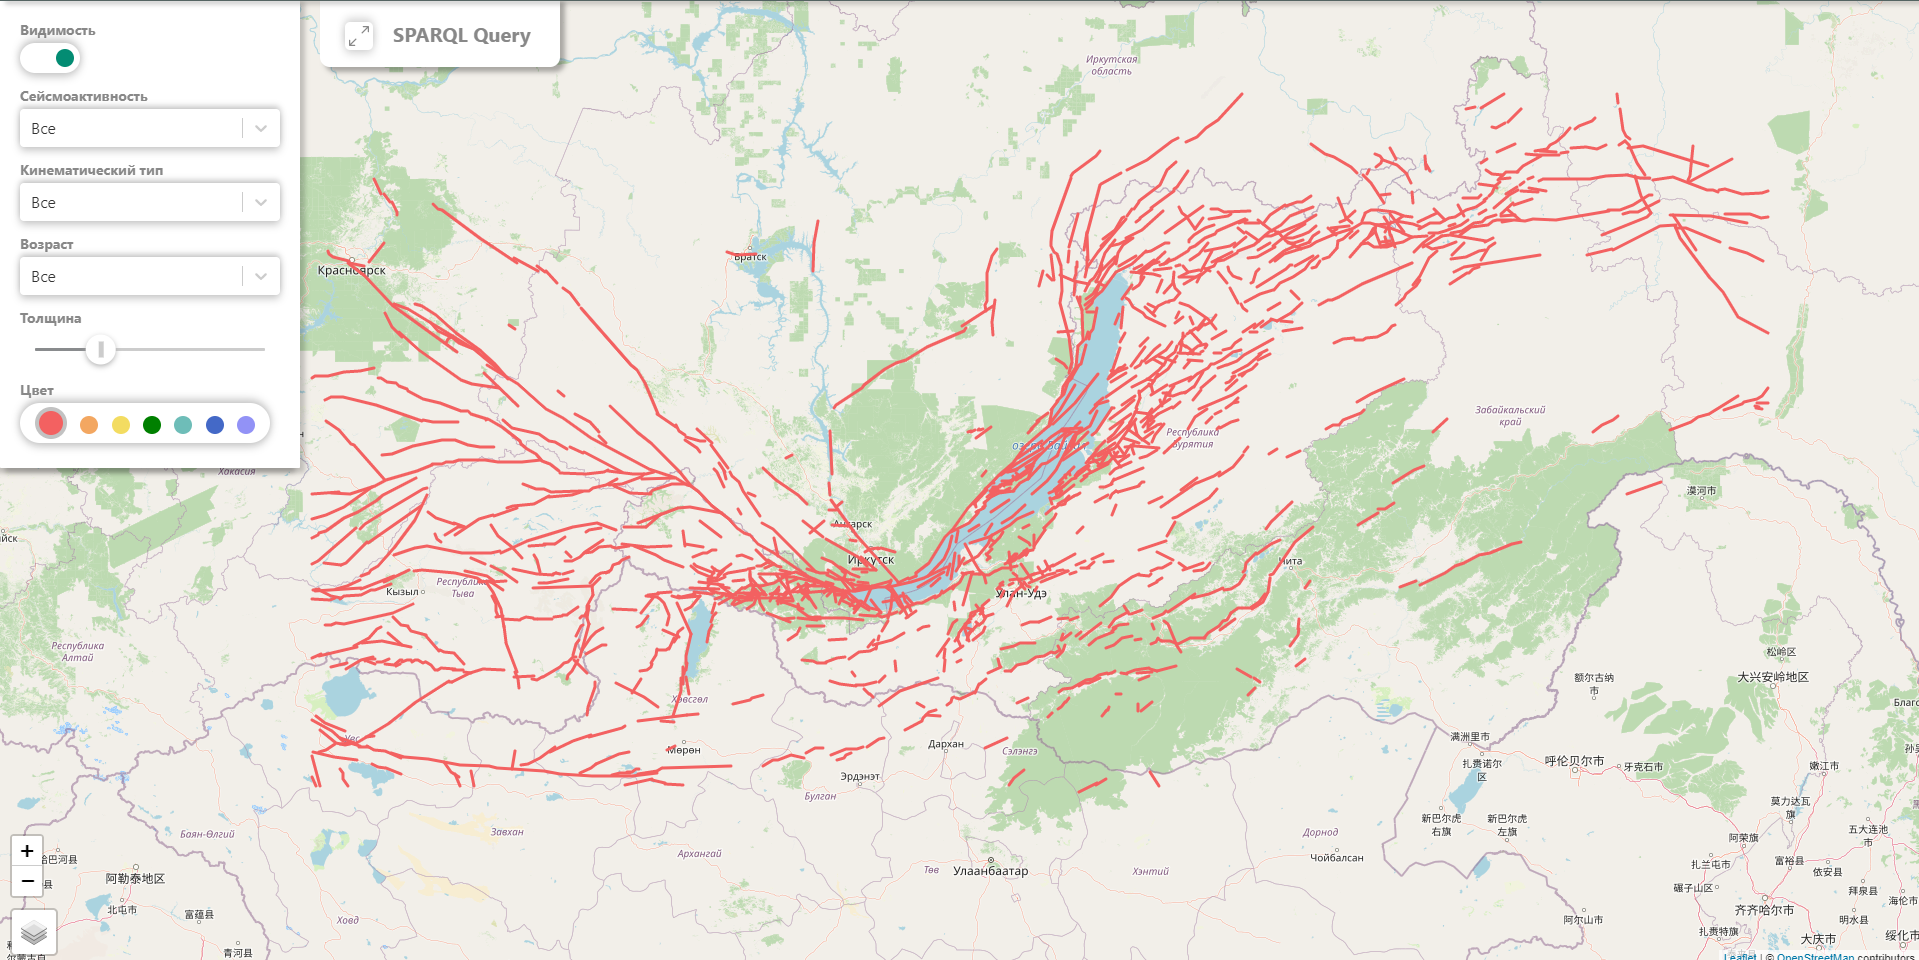
\includegraphics[width=\linewidth]{faults-leaflet-all.png}
\end{frame}

\begin{frame}
  \frametitle{WEB-GIS viewer of active faults of East Siberia}
  \centering
  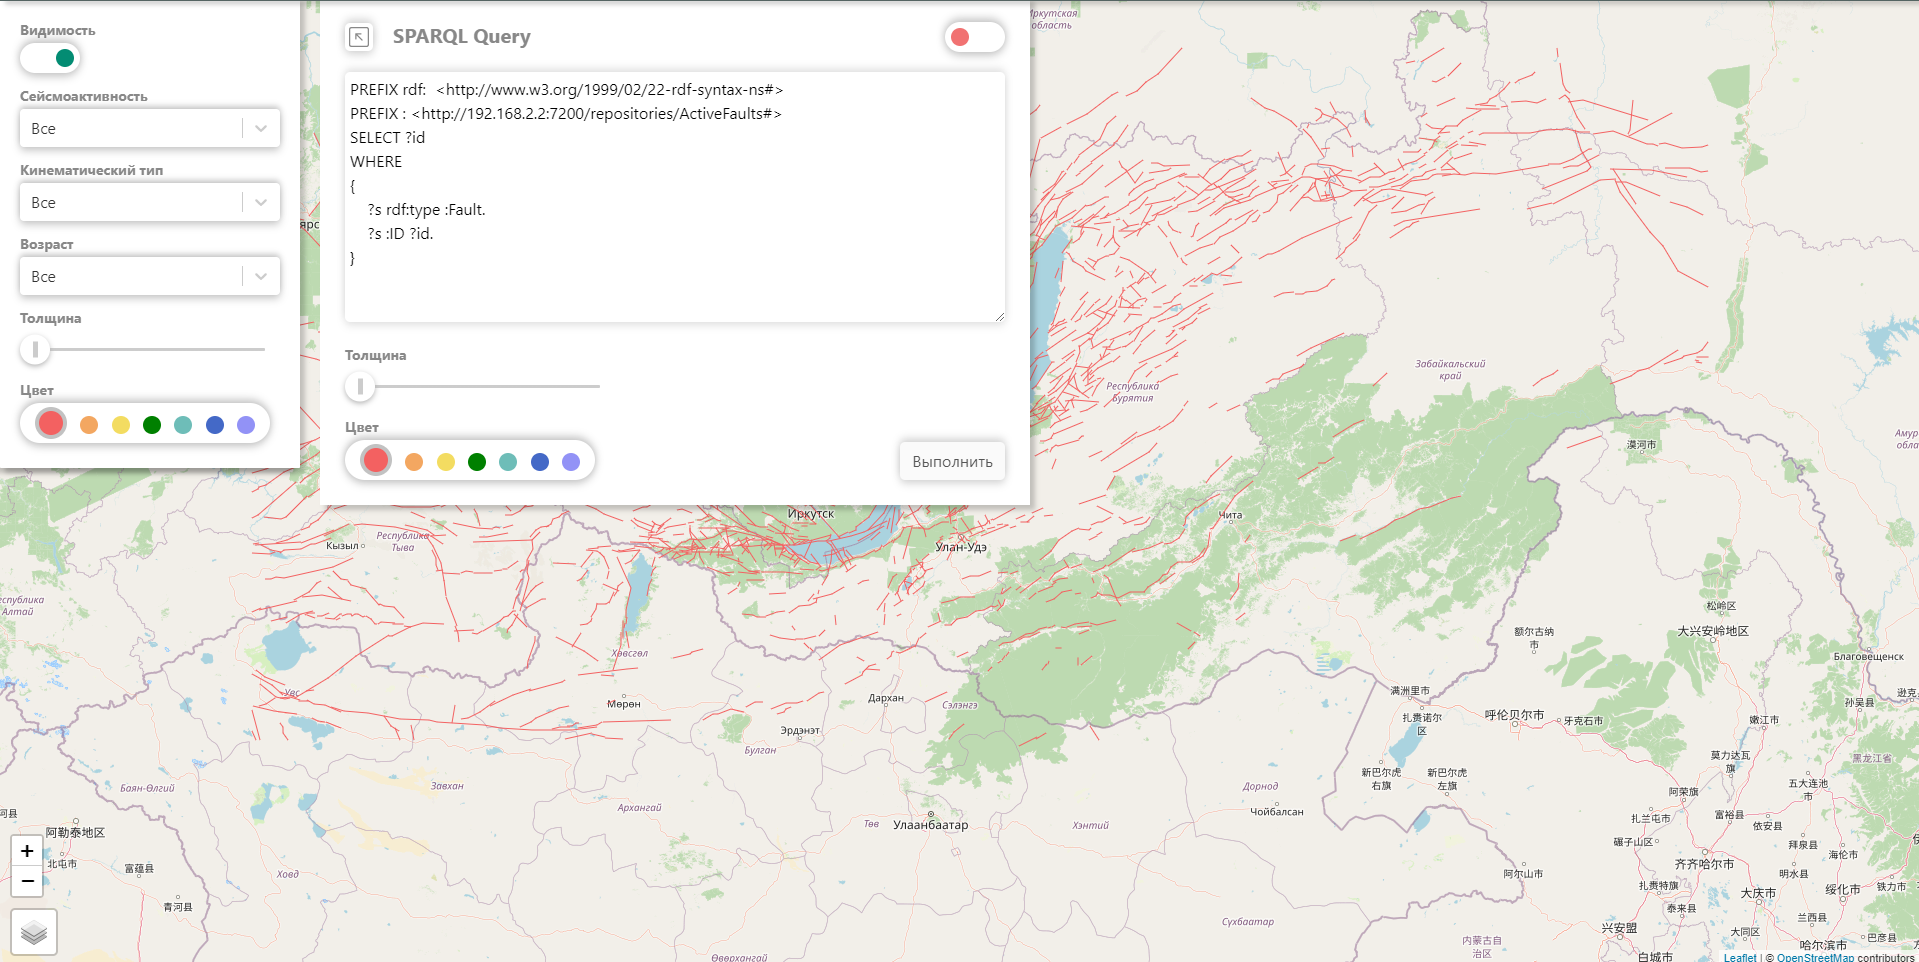
\includegraphics[width=\linewidth]{faults-leaflet-sparql.png}
\end{frame}

\begin{frame}
  \frametitle{WEB-GIS viewer of active faults of East Siberia}
  \centering
  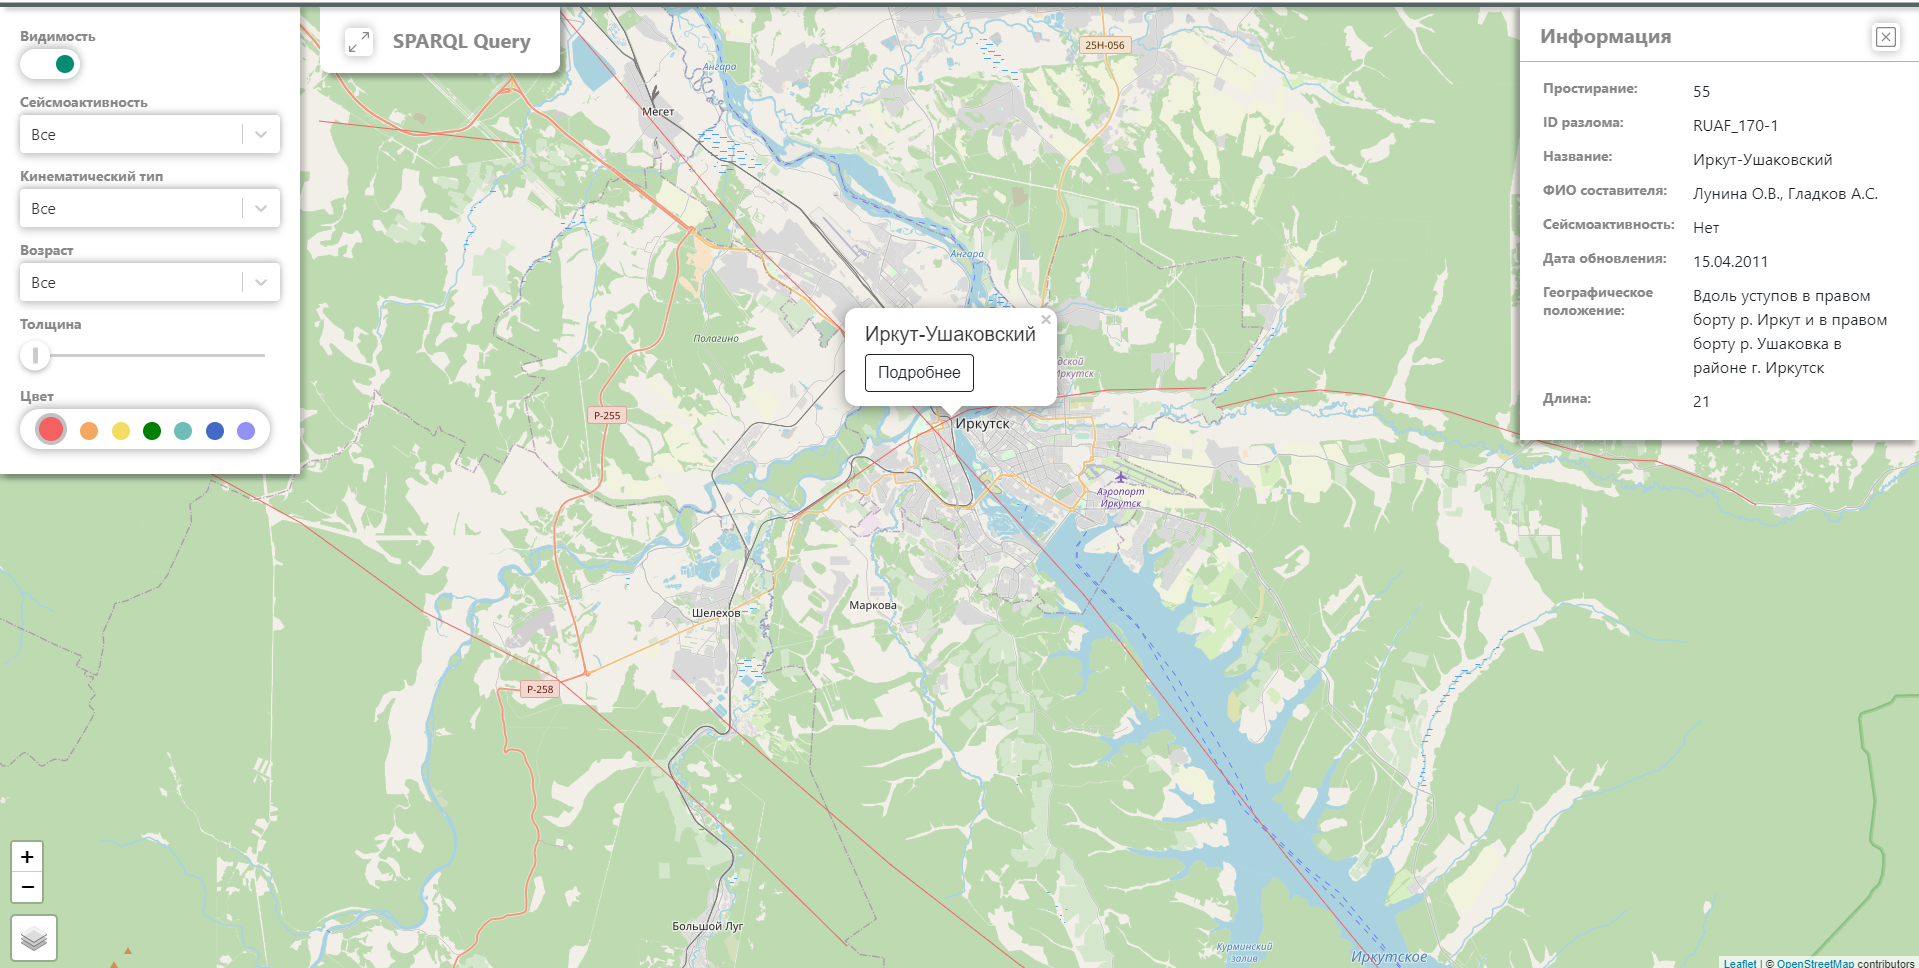
\includegraphics[width=\linewidth]{faults-leaflet-doc.png}
\end{frame}

\begin{frame}
  \frametitle{Ontology (vocabulary) of database of faults}
  \centering
  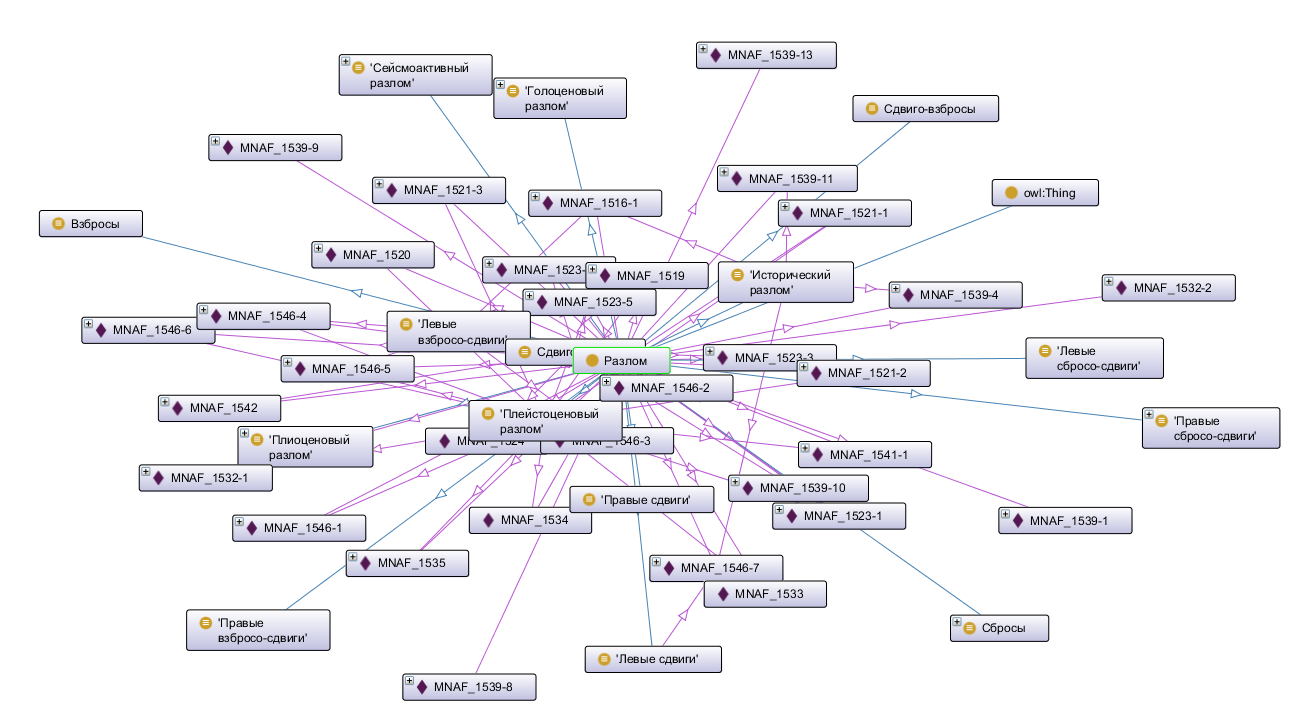
\includegraphics[width=\linewidth]{faults-ontology-view.png}
\end{frame}

\begin{frame}
  \frametitle{Used technologies}
  The applications were constructed using contemporary packages.
  \begin{itemize}
  \item Topological basis (TB) is loaded from \url{openstreetmap.org} by
  \item Leaflet JavaScript module wrapped in
  \item a React.js component.
  \item As vocabulary data source GraphDB and Apache Jena was used.
  \item WEB-GIS application state dynamics is implemented with Redux.
  \item Fault shapes is represented as JSON objects.
  \end{itemize}
\end{frame}

\begin{frame}
  \frametitle{Publishing Geodata LOD in context dependent pages}
  The project\footnote{Adam Iwaniak, Marta Leszczuk, Marek Strzelecki, Francis Harvey, Iwona Kaczmarek. A Novel Approach for Publishing Linked Open Geodata from National Registries with the Use of Semantically Annotated Context Dependent Web Pages. International Journal of Geo-Information. 6, 252, 2017. \doi{10.3390/ijgi6080252}} goal is to convert existing GIS data into explicit knowledge, thus, forming a Spatial Data Infrastructure (SDI).
  \begin{itemize}
  \item Integrate existing geoportal data into a KB, including dynamic data
  \item Geoportal data must be LOD, \emph{e.g.}, HTML is enriched with RDFa
  \item Relation interpreters implemented as Expert systems (``building near forest'')
  \item Semantic enrichment of raw data to make it more usable/discoverable
  \item Targeting to GeoSPARQL (sfIntersects, sfOverlaps, sfTouches, sfWithin, sfContains))
  \item Metadata inference from the data source properties
  \item Test application is to integrate public services data in Mazowieckie Voivodeship of Poland, queries are realized by a limited set of keywords
  \end{itemize}
\end{frame}

\begin{frame}
  \frametitle{Publishing Geodata LOD in context dependent pages}
  % Figure of GIS and SPARQL query
  \centering
  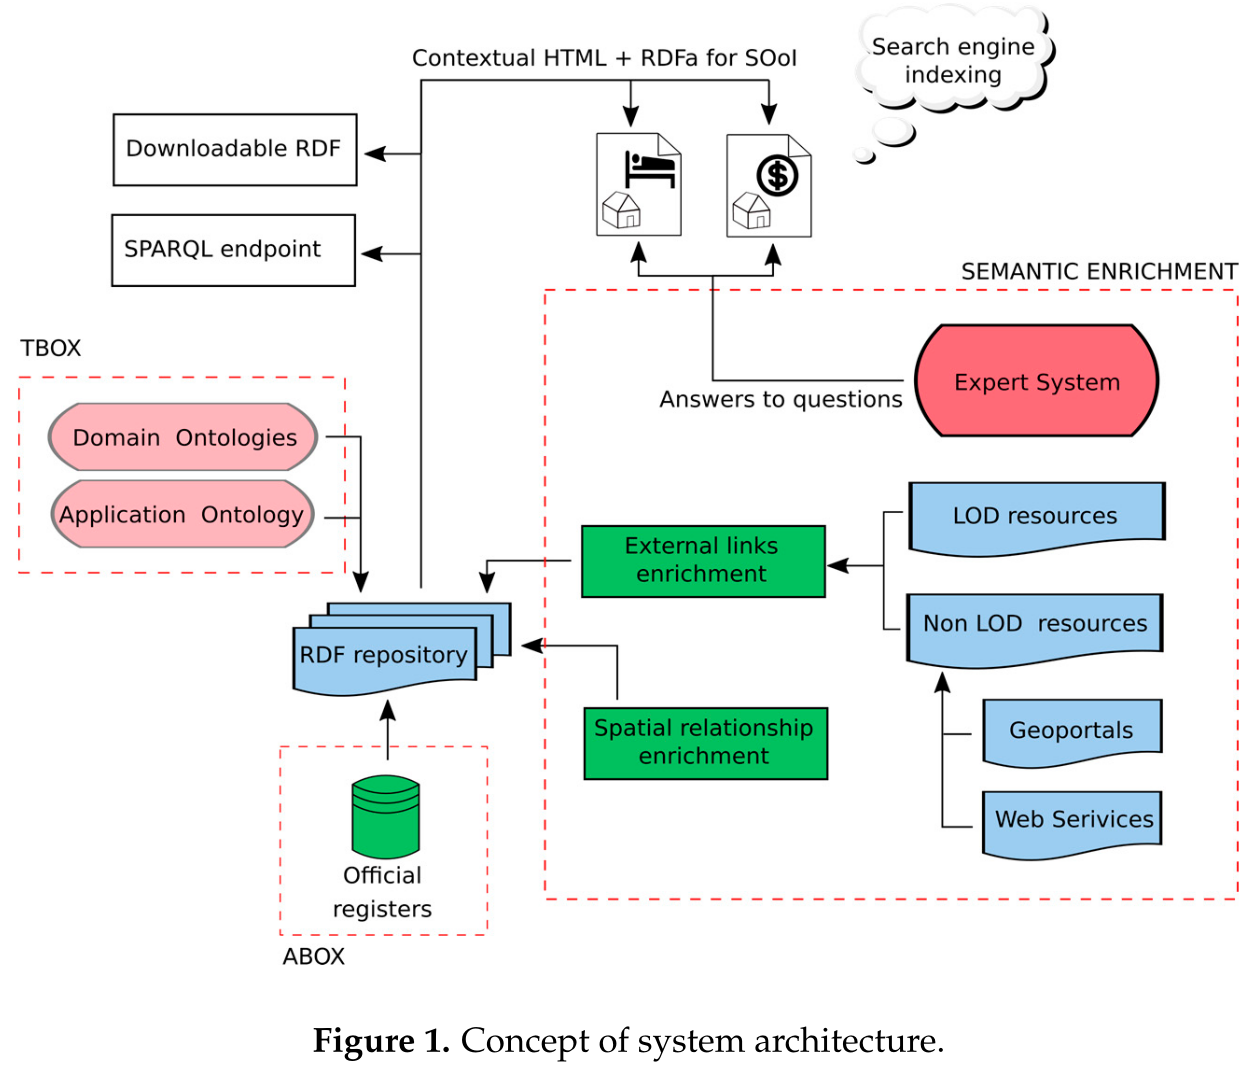
\includegraphics[width=0.8\linewidth]{integrating-tech.png}
\end{frame}

\begin{frame}
  \frametitle{Enriching and improving the quality of linked data
with GIS}
  % Figure of GIS and SPARQL query
  \begin{center}
   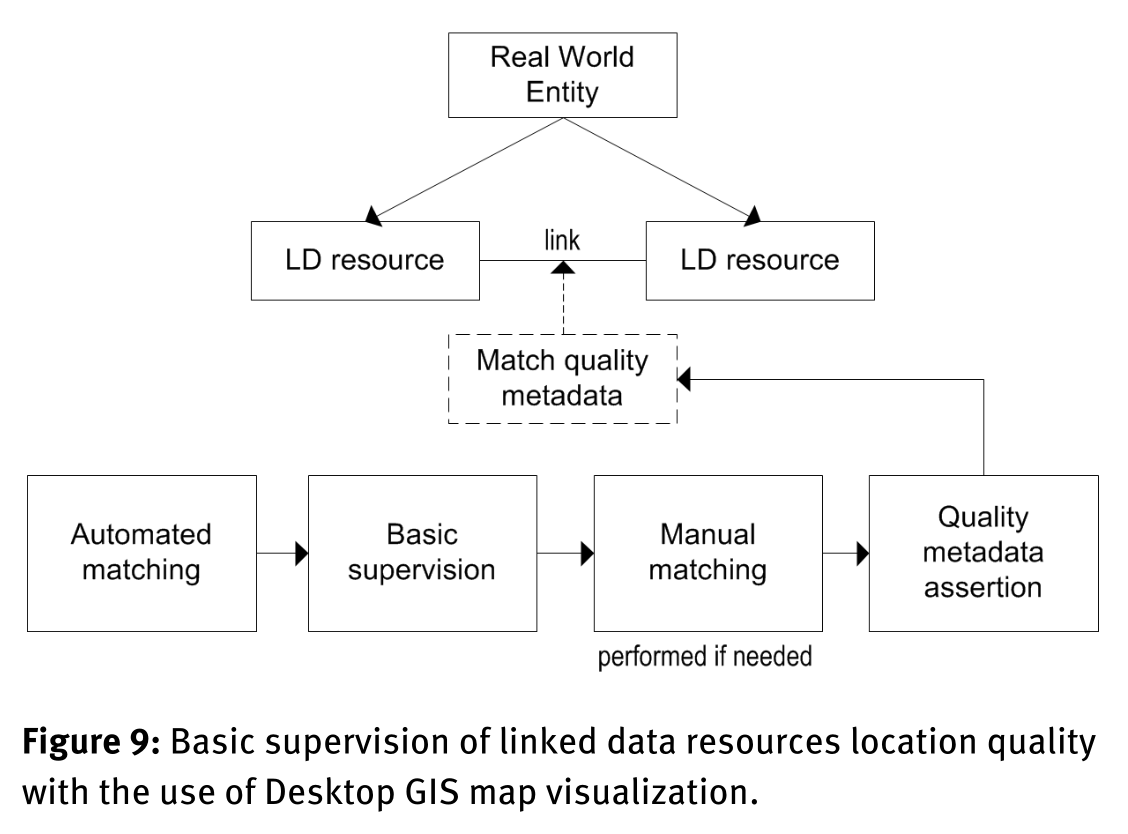
\includegraphics[width=0.7\linewidth]{deducing-rels.png}
 \end{center}
 From an early work\footnote{Adam Iwaniak, Iwona Kaczmarek, Marek Strzelecki, Jaromar Lukowicz, Piotr Jankowski. Enriching and improving the quality of linked data with GIS. \doi{10.1515/geo-2016-0c020}}.
\end{frame}

\begin{frame}
  \frametitle{Enriching and improving the quality of linked data...}

  \begin{center}
   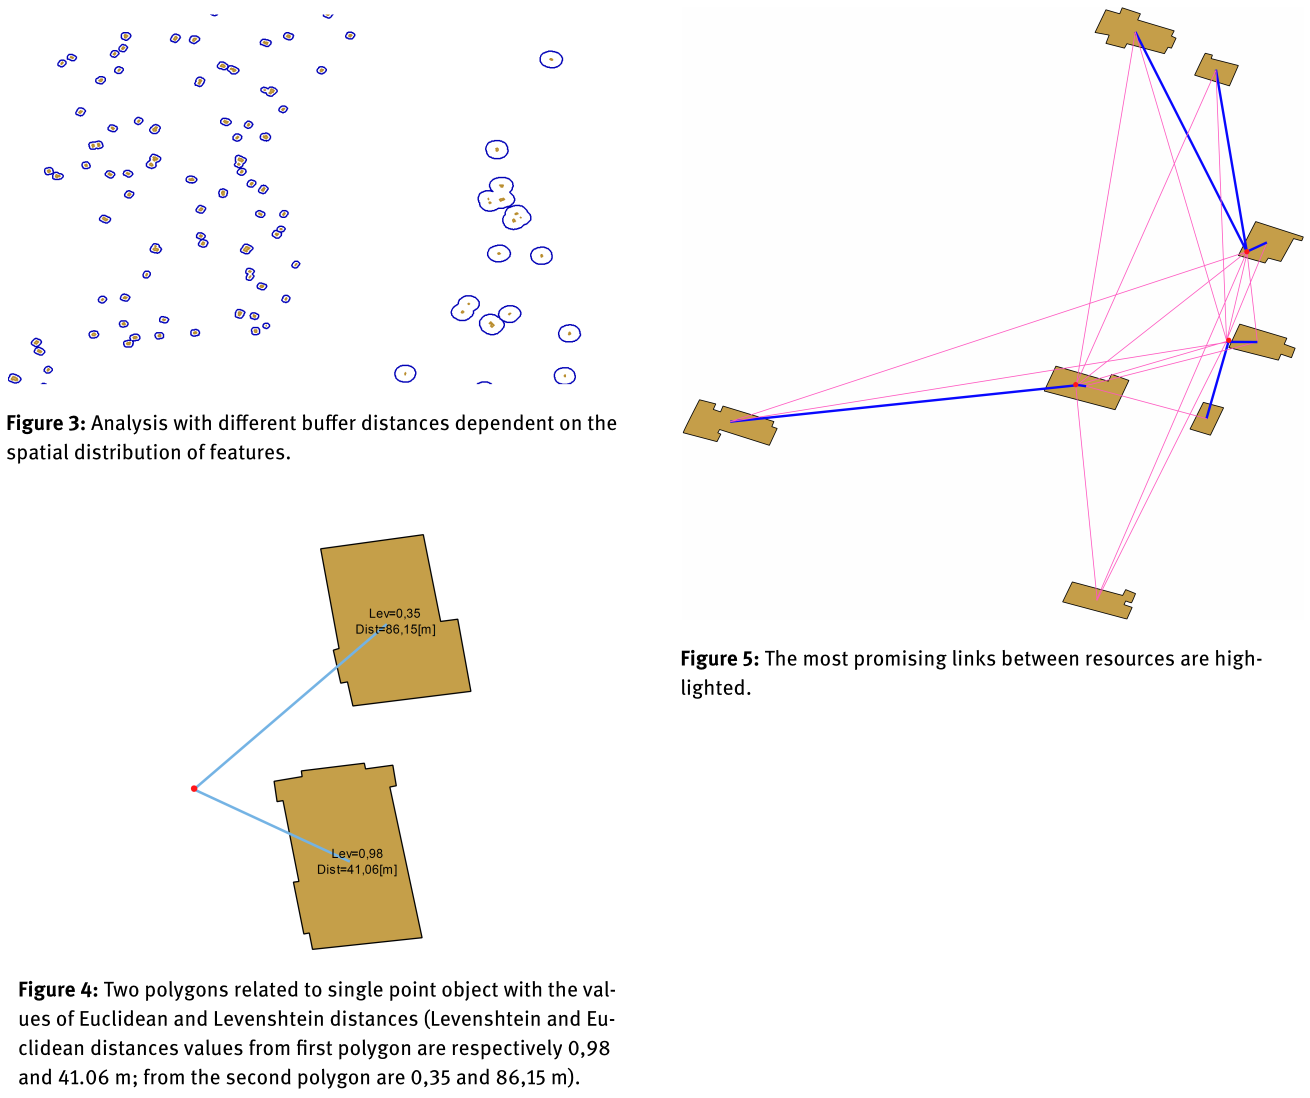
\includegraphics[width=0.8\linewidth]{joining-objs.png}
 \end{center}
\end{frame}

\begin{frame}
  \frametitle{Publishing Geodata LOD in context dependent pages}
  % Figure of GIS and SPARQL query
  \centering
  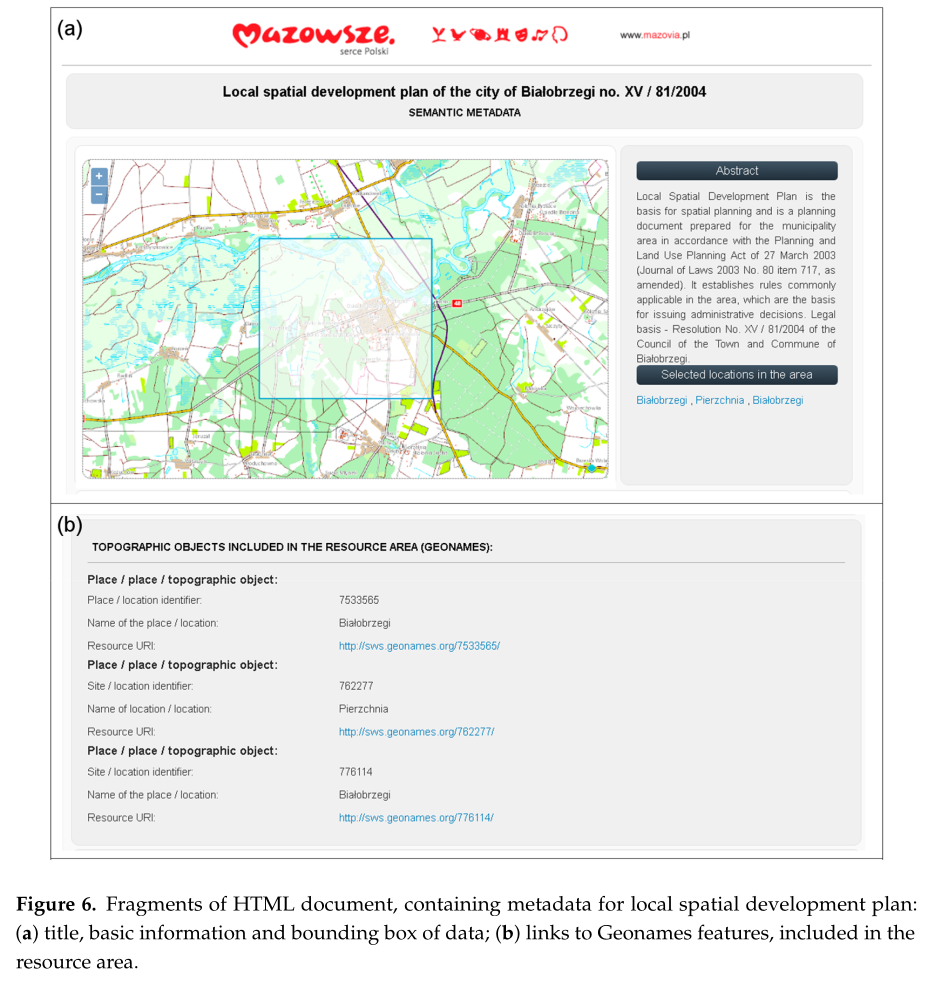
\includegraphics[width=0.7\linewidth]{integrating-og.png}
\end{frame}


% \begin{frame}
%   \frametitle{Related Works: Publishing Geodata LOD in context dependent pages}
%   % figure 1 of Concept of system architecture
%   % figure 2 HTML example
% \end{frame}

\begin{frame}\centering
  \Large Existing geological GIS resources
\end{frame}


\begin{frame}
  \frametitle{Active faults of Japan islands}
  % Figure of GIS and SPARQL query
  \centering
  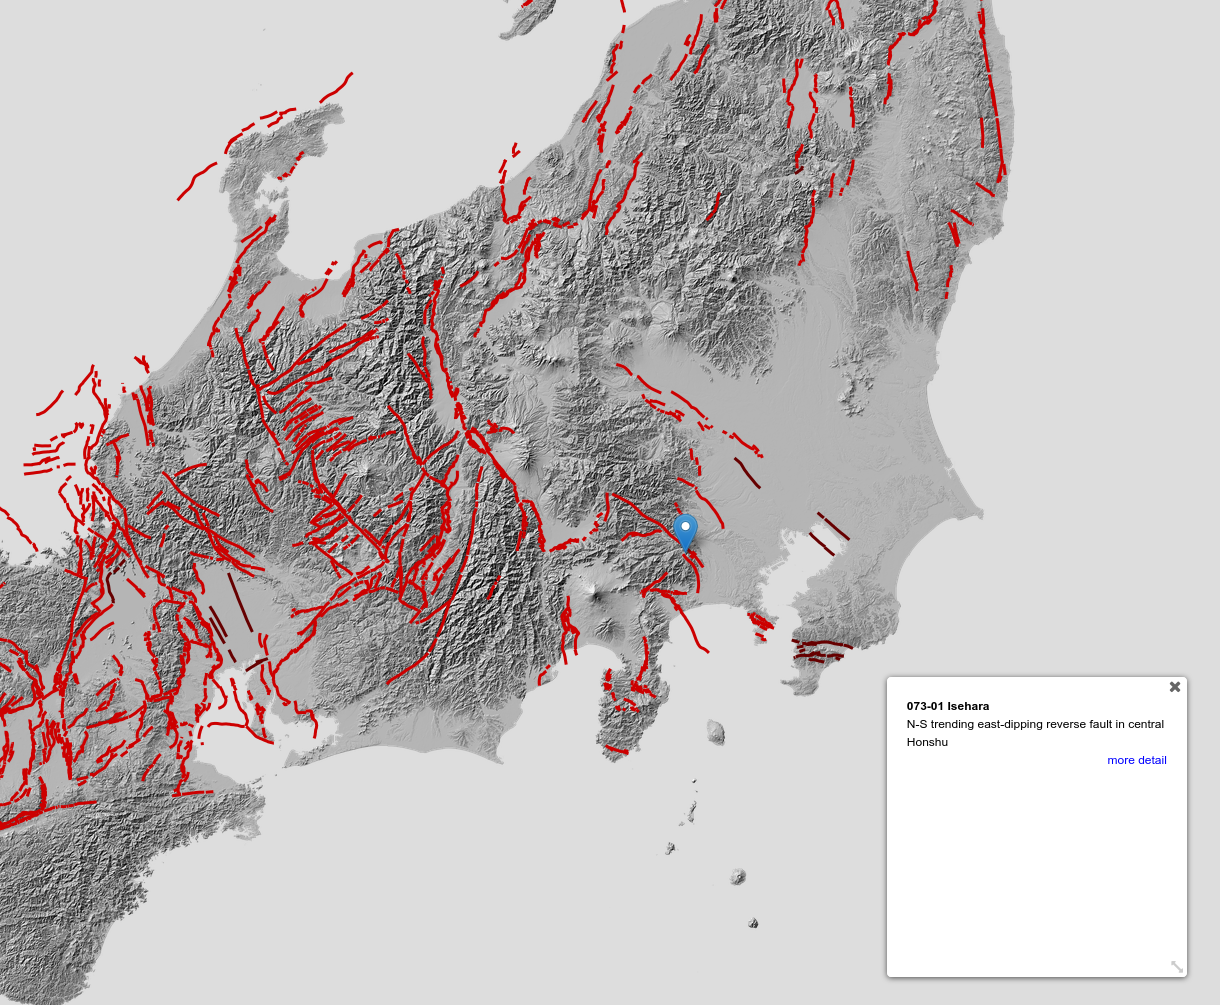
\includegraphics[width=\linewidth]{japan.png}
\end{frame}

\begin{frame}
  \frametitle{Active fault of Italian Peninsula}
  % Figure of GIS and SPARQL query
  \centering
  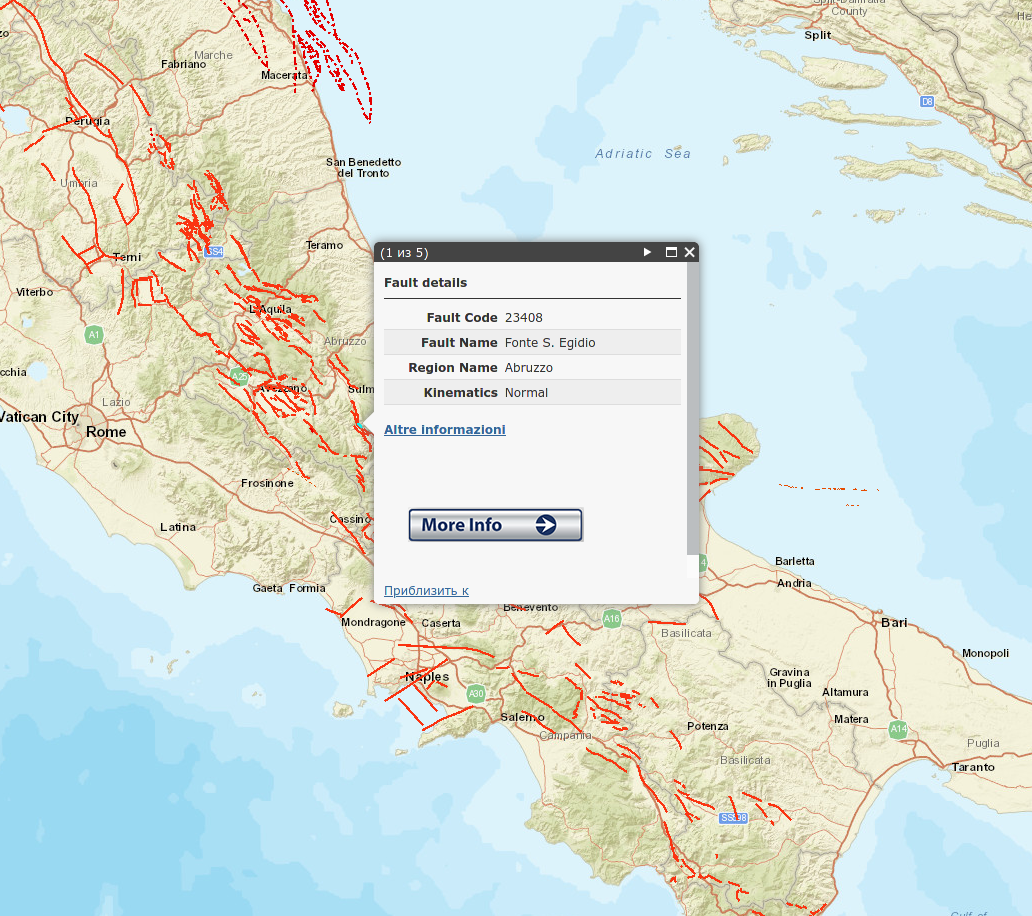
\includegraphics[width=\linewidth]{italy-1.png}
\end{frame}

\begin{frame}
  \frametitle{Active fault of Italian Peninsula}
  % Figure of GIS and SPARQL query
  \centering
  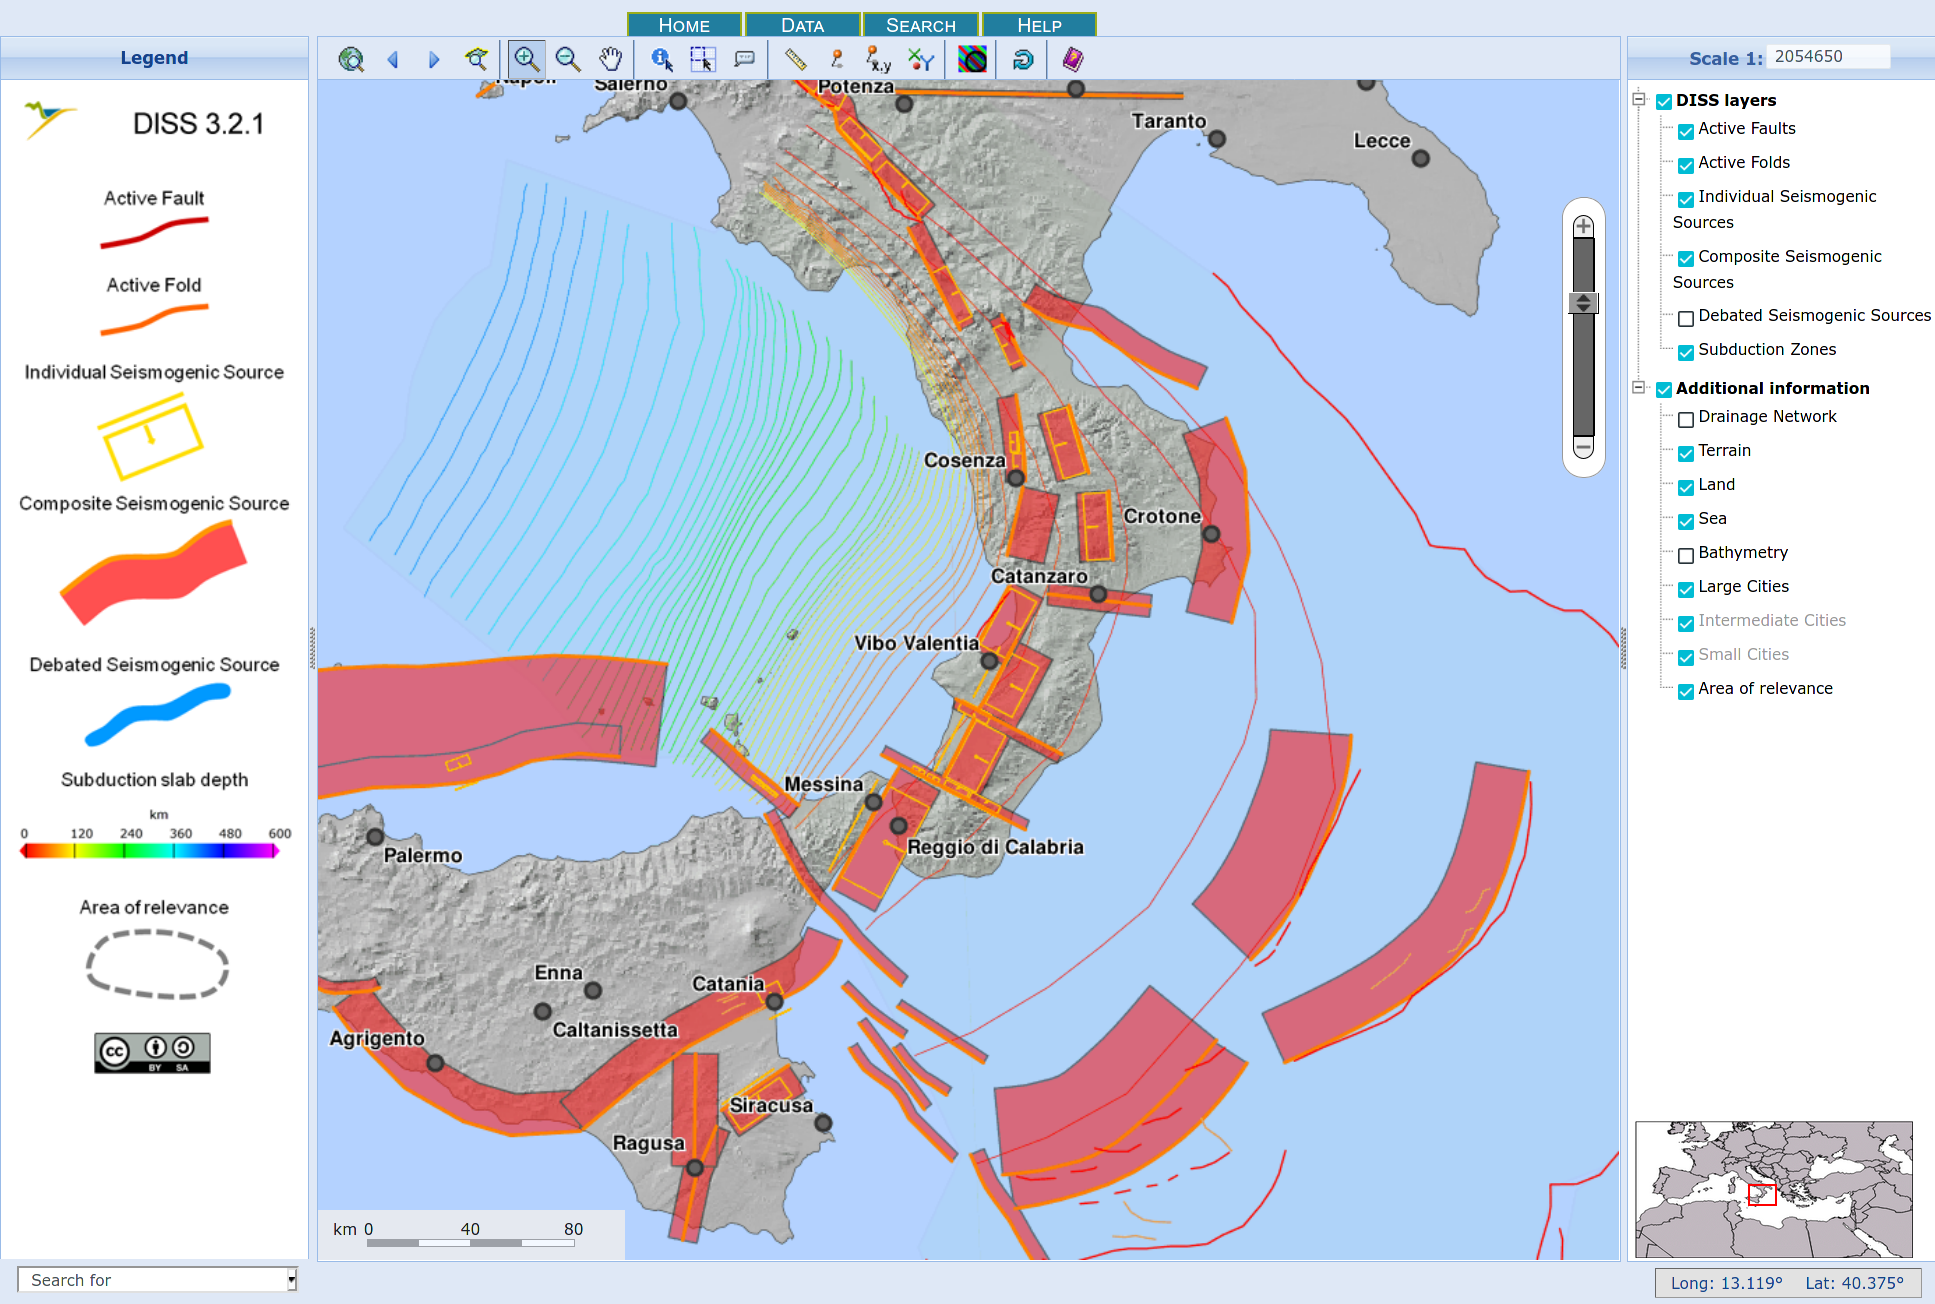
\includegraphics[width=\linewidth]{italy-2.png}
\end{frame}

\begin{frame}\centering
  \Large Resources to be presented
\end{frame}

\begin{frame}
  \frametitle{Active faults of the South of East Siberia}
  % Screenshot of the system
  \centering
  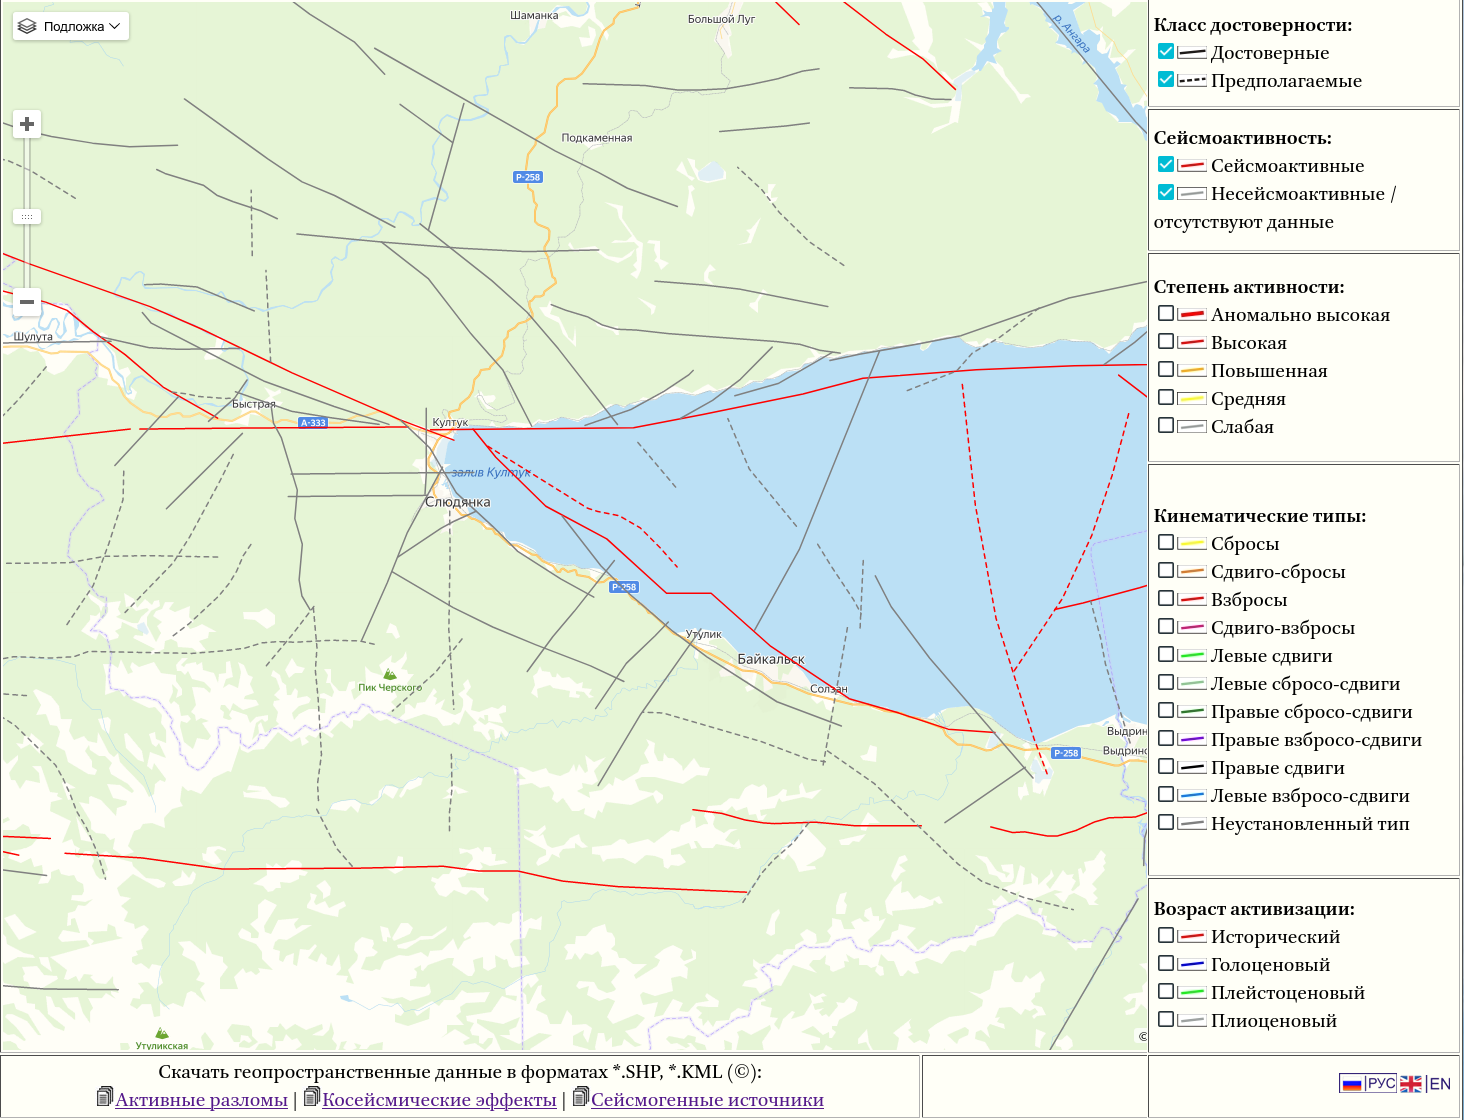
\includegraphics[width=0.9\linewidth]{activetectonics.png}
  \url{http://http://activetectonics.ru/}
\end{frame}

\begin{frame}
  \frametitle{Resources to be presented: Active faults of the South of
    East Siberia}
  The fault data\footnote{Oksana V. Lunina.  The digital map of the pliocene quaternary crustal faults in the southern east siberia and the adjacent northern Mongolia. Geodynamics \& Tectonophysics. 2016. 7(3):407-434. \doi{10.5800/GT-2016-7-3-0215}
} have the following properties:
  \begin{itemize}
  \item Faults are the objects having linear projection on the surface, and a depth and a slope in the lithosphere
  \item Various geological events are also subjects of presentation
  \item Any object accompanied by various valued characteristics having also characteristics, \emph{e.g.}, unit name, measurement precision and related publications
  \item Images, tables, expedition trails are also used as auxiliary materials.
  \end{itemize}
\end{frame}

\begin{frame}[fragile]
  \frametitle{Database Structure}
  \begin{columns}\tiny
    \begin{column}{0.5\linewidth}
\begin{verbatim}
!table
!version 300
!charset WindowsCyrillic

Definition Table
  Type NATIVE Charset "WindowsCyrillic"
  Fields 72
    ID Char (15) Index 1 ;
    Name Char (40) Index 2 ;
    Location Char (250) Index 3 ;
    Strike Char (10) Index 4 ;
    Strike_Q Char (2) ;
    Dip_azimuth Char (10) Index 5 ;
    Dip_azimuth_Q Char (2) ;
    Dip_angle Char (10) Index 6 ;
    Dip_angle_Q Char (2) ;
    Length_km Char (10) Index 7 ;
    Length_Q Char (2) ;
    Depth_km Char (10) Index 8 ;
    Depth_Q Char (2) ;
    Width_damage_zone_km Char (10) Index 9 ;
    Width_damage_zone_Q Char (2) ;
    Slip_sense Char (30) Index 10 ;
    Slip_sense_Q Char (2) ;
    Slip_sense_Index Decimal (2, 0) ;
    Total_Cenozoic_lateral_slip_m Char (20) ;
    Total_Cenozoic_lateral_slip_Q Char (2) ;
    Total_Cenozoic_vertical_slip_m Char (20) ;
    Total_Cenozoic_vertical_slip_Q Char (2) ;
    Reliability_class Decimal (1, 0) Index 11 ;
    Geomorphological_features Char (250) ;
    Geomorphological_grade Integer Index 12 ;
    Geophysical_features Char (254) ;
    Geophysical_grade Integer Index 13 ;
    Engineering_geological_features Char (254) ;
    Engineering_geological_grade Integer Index 14 ;
    Gydrogeological_features Char (200) ;
    Gydrogeological_grade Integer Index 15 ;
    Meteorological_features Char (50) ;
    Meteorological_grade Integer Index 16 ;
\end{verbatim}
    \end{column}
    \begin{column}{0.5\linewidth}
\begin{verbatim}

    Structural_geological_features Char (254) ;
    Structural_geological_grade Integer Index 17 ;
    Paleoseismological_features Char (254) ;
    Paleoseismological_grade Integer Index 18 ;
    Seismological_features Char (100) ;
    Seismological_grade Integer Index 19 ;
    Slip_rate_features Char (10) ;
    Slip_rate_grade Integer Index 20 ;
    Total_activity_grade Decimal (4, 0) Index 21 ;
    Activity_degree Char (25) Index 22 ;
    Last_activation_age Char (30) Index 23 ;
    Last_activation_age_index Decimal (1, 0) Index 24 ;
    Last_historical_earthquake Char (150) Index 25 ;
    Last_historical_earthquake_Q Char (2) ;
    Absolute_deformation_age Char (254) ;
    Absolute_deformation_age_Q Char (2) ;
    Vertical_max_slip_per_event_m Float ;
    Vertical_max_slip_per_event_Q Char (2) ;
    Lateral_max_slip_per_event_m Float ;
    Lateral_max_slip_per_event_Q Char (2) ;
    Total_max_slip_per_event_m Float ;
    Total_max_slip_per_event_Q Char (2) ;
    Slip_rate_mm_year Char (30) ;
    Slip_rate_Q Char (2) ;
    Averaged_slip_rate_mm_year Float ;
    Averaged_slip_rate_Q Char (2) ;
    Recurrence_interval Char (10) Index 26 ;
    Recurrence_interval_Q Char (2) ;
    Potential_Ms_max Float ;
    Potential_Ms_max_Q Char (2) ;
    Potential_Mw_max Float ;
    Potential_Mw_max_Q Char (2) ;
    Elapsed_time_years Char (10) ;
    Elapsed_time_Q Char (2) ;
    Associated_CSS Char (25) ;
    Associated_IGGSS Char (50) ;
    Seismic_activity_of_fault Char (3) ;
    Compiler Char (50) ;
    Date Char (10) ;
\end{verbatim}
    \end{column}
  \end{columns}
\end{frame}

\begin{frame}
  \frametitle{The pollutions of Olkhon Island}
   % Generate a map from the existing data
  \centering
   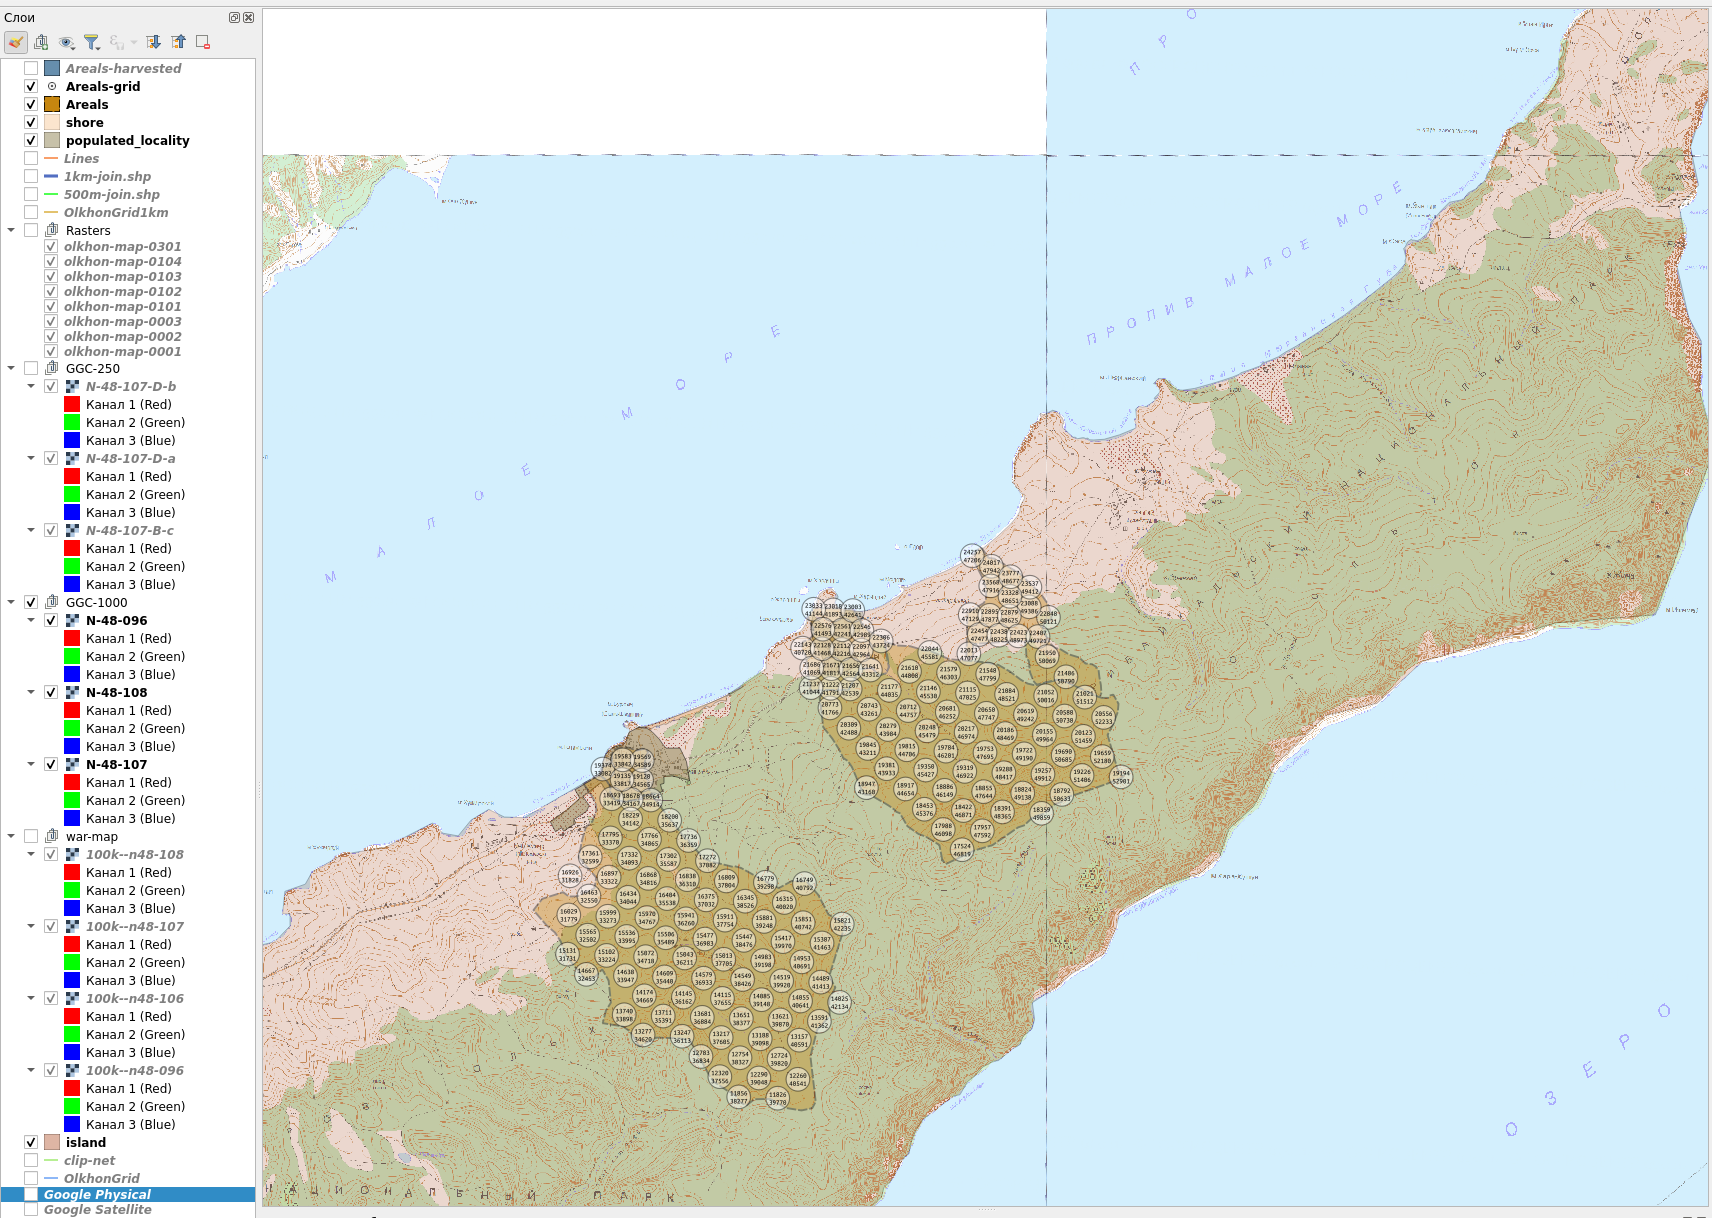
\includegraphics[width=\linewidth]{olkhon-gis.png}
\end{frame}

\begin{frame}
  \frametitle{System architecture}
  \centering
  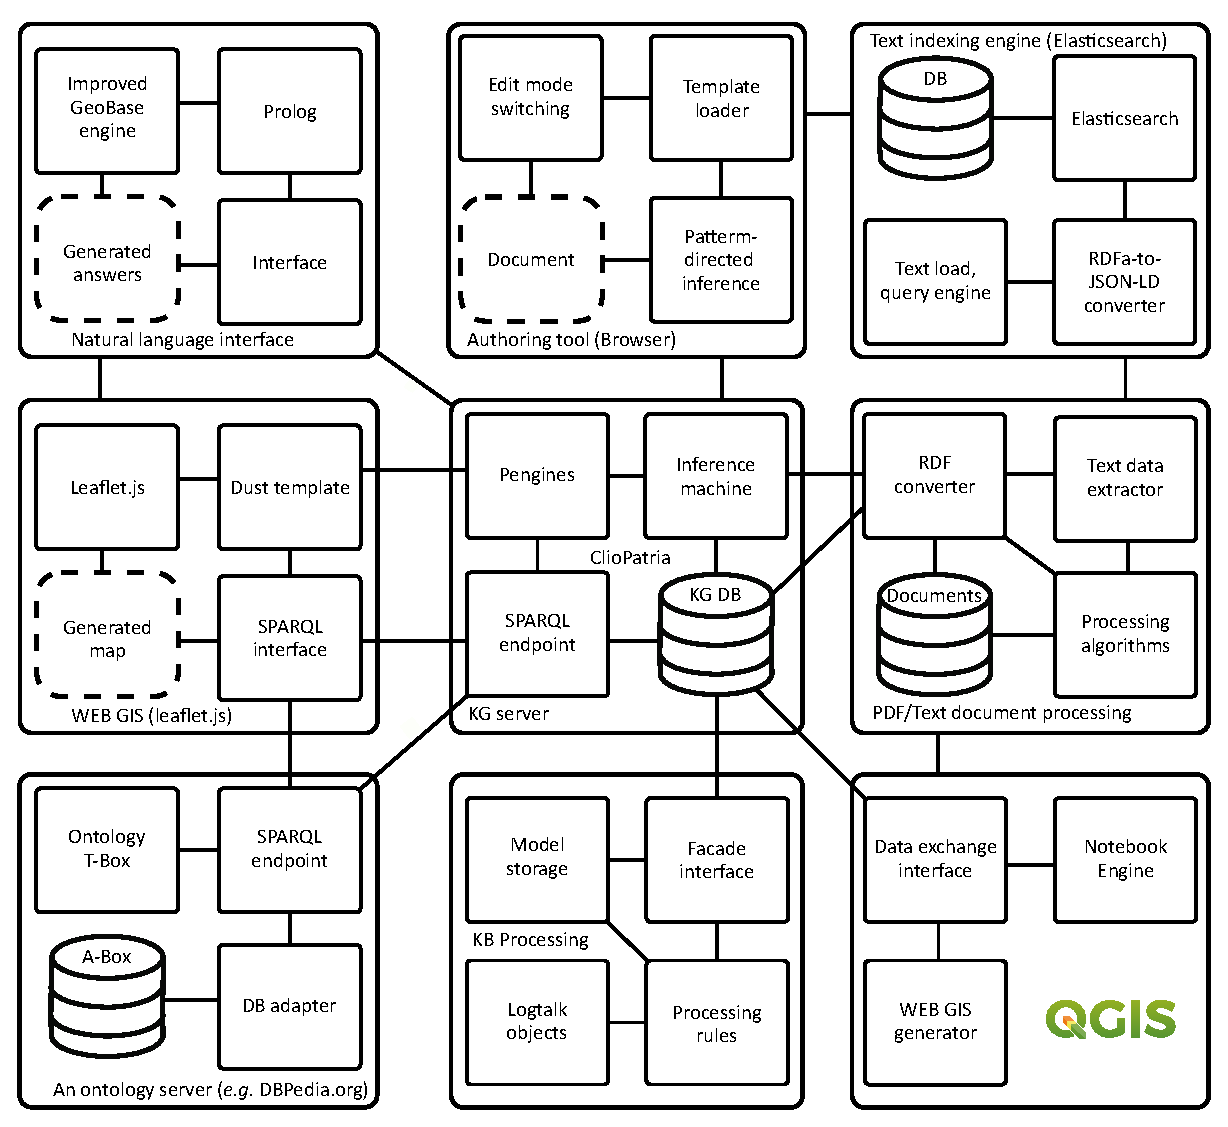
\includegraphics[width=0.8\linewidth]{architecture.pdf}
\end{frame}

\begin{frame}
  \frametitle{Leaflet}
  \centering
  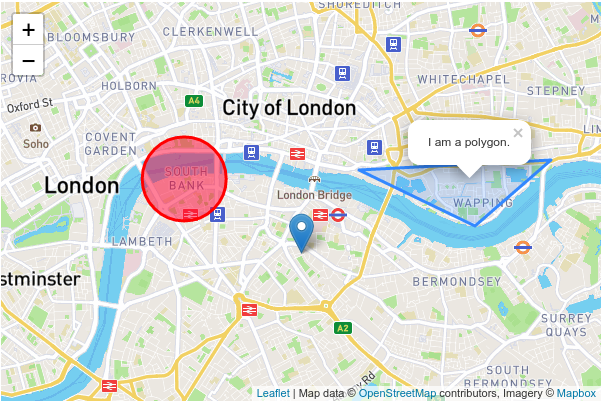
\includegraphics[width=0.8\linewidth]{leaflet.png}
\end{frame}

\begin{frame}
  \frametitle{Conclusion}
  The following results have been obtained as for today:
  \begin{itemize}
  \item A short review of similar\& basic projects has been carried out
  \item An experience has been obtained in usage of standardized ontologies and SW techniques
  \item The project is relevant in sense of application of standards in data publishing
  \item There are technologies allowing to implement such services, they're mostly web-oriented
  \item Application of the reviewed technologies will extend the research possibilities
  \end{itemize}
  The results were obtained within the framework of the State Assignment of the Ministry of Education and Science of the Russian Federation for the project ``Methods and technologies of cloud-based service-oriented platform for collecting, storing and processing large volumes of multi-format interdisciplinary data and knowledge based upon the use of artificial intelligence, model-guided approach and machine learning''. Some results were obtained using the facilities of the Centre of collective usage ``Integrated information network of Irkutsk scientific educational complex''.
\end{frame}

\begin{frame}
  \frametitle{External links}
  The presentation URL
  \begin{columns}
    \begin{column}{0.3\textwidth}
      
\includegraphics[width=1\linewidth]{talk.pdf}
    \end{column}
    \begin{column}{0.7\textwidth}
      \url{https://raw.githubusercontent.com/eugeneai/paper-2021-iwci/main/talk-IWCI-2021-03-30.pdf}
    \end{column}
  \end{columns}
  \vspace{3em}
  \begin{center}
  \Large Thank You!
\end{center}
\end{frame}

\maketitle

\begin{frame}
  \frametitle{External links}\footnotesize
  \begin{thebibliography}{99}
\bibitem{hogan} Aidan Hogan, Eva Blomqvist, Michael Cochez, Claudia D’Amato \emph{et al}. Knowledge Graphs. \url{https://arxiv.org/abs/2003.02320v5}
\bibitem{lgd} Claus Stadler, Jens Lehmann, Konrad Höffner, Sören Auer. LinkedGeoData: A core for a web of spatial open data. Semantic Web 3 (2012) 333–354. \doi{10.3233/SW-2011-0052}

\bibitem{iwaniak1} Adam Iwaniak, Iwona Kaczmarek, Marek Strzelecki, Jaromar Lukowicz, Piotr Jankowski. Enriching and improving the quality of linked data with GIS. \doi{10.1515/geo-2016-0c020}

\bibitem{iwaniak17} Adam Iwaniak, Marta Leszczuk, Marek Strzelecki, Francis Harvey, Iwona Kaczmarek. A Novel Approach for Publishing Linked Open Geodata from National Registries with the Use of Semantically Annotated Context Dependent Web Pages. International Journal of Geo-Information. 6, 252, 2017. \doi{10.3390/ijgi6080252}

\bibitem{abid} Tarek Abid, Hafed Zarzour. Integrating Linked Open Data in Geographical
Information System. International Conference on Information Technology for Organization Development. 2014.

\bibitem{geolink} Michelle Cheatham, Adila Krisnadhi, Reihaneh Amini, Pascal Hitzler, \emph{et al} (2018) The GeoLink knowledge graph, Big Earth Data, 2:2, 131-143, \doi{10.1080/20964471.2018.1469291}

\bibitem{lunina} Oksana V. Lunina.  The digital map of the pliocene quaternary crustal faults in the southern east siberia and the adjacent northern Mongolia. Geodynamics \& Tectonophysics. 2016. 7(3):407-434. \doi{10.5800/GT-2016-7-3-0215}
\end{thebibliography}
\end{frame}

\begin{frame}
  \begin{center}
  \Large Auxiliary materials
\end{center}
\end{frame}

\begin{frame}
  \frametitle{Technologies used (open source)}
  Python-3.x.x (\url{http://python.org})\\
  ZCA (\url{https://muthukadan.net/docs/zca.html})\\
  SWIG (\url{http://swig.org/})\\
  SWI-Prolog (\url{https://www.swi-prolog.org/})\\
  Logtalk (\url{https://logtalk.org/})\\
  ClioPatria (\url{https://cliopatria.swi-prolog.org/home})\\
  Virtuoso Open Source Edition (http://vos.openlinksw.com/owiki/wiki/VOS)\\
  Pengines (\url{https://pengines.swi-prolog.org/docs/index.html})\\
  LOV (\url{https://lov.linkeddata.es/dataset/lov/})\\
  Elastic Search (\url{https://www.elastic.co/})\\
  Kyotocabinet (\url{https://fallabs.com/kyotocabinet/})\\
  DBPedia (\url{https://wiki.dbpedia.org/})\\
  % Mothur (\url{https://mothur.org/}),\\
  % Galaxy (\url{https://usegalaxy.org/}),\\
  % R (\url{https://www.r-project.org/}), \\
  Dust.js (\url{https://akdubya.github.io/dustjs/})\\
  QGIS (\url{https://qgis.org/ru/site/})\\
  TabbyDOC (\url{http://td.icc.ru/})\\
  GeoBase (\url{https://github.com/eugeneai/geobase})\\
  Authoring Tool (\url{https://github.com/isu-enterprise/isu.college})
\end{frame}

% \begin{frame}[fragile]
%   \frametitle{Semantic Web technologies in representation of models
%     during transformation}
%   \begin{itemize}
%   \item Assimilates experience of domain basic researches trending to standardization;
%   \item Regular set of triples denote a graph (T-Box, A-Box);
%   \item Standard vocabularies are formally described (\verb|rdfs:domain|, \verb|rdfs:range|);
%   \item Supported with most programming systems (libraries, inference engines, SPARQL);
%   \item RDF has a way of global element identification, \emph{i.e.} we can refer the same object from different software systems;
%   \item SWI-Prolog supports direct queries to a graph, as well as interpreting some predicates (\verb|rdfs:label|, \verb|dc:title|), wraps sparse RDF structure into a predicate arguments; ontological server ClioPatria;
%   \item There is simple way of data security implementation (\verb|rdfs:seeAlso|);
%   \item By means of Semantic Web \& LOD we are able to organize data transfer between heterogeneous information systems.
%   \end{itemize}
% \end{frame}

\begin{frame}
  \frametitle{Used ontologies}

  Standardized ontologies

  \begin{itemize}
  \item Friend-of-a-friend (\textbf{foaf}) for agent information: individuals, legal entities, program agents
  \item Provenance (\textbf{prov}) for making references between documents
  \item Dublin Core (\textbf{dc}) for published resource metadata mark up
  \item DBPedia resource (\textbf{dbr}) to refer external classes and instance objects
  \item Schema.org (\textbf{schema}) for Google, Yandex, Yahoo, \emph{etc}. searchable objects, structural elements
  \item The Bibliographic Ontology (\textbf{bibo}) used for literature reference
  \item Open annotation (\textbf{oa}) as an ``bookmark'' ontology
% Namespaces
  \item LinkedGeoData A-Box (\textbf{lgd}) % http://linkedgeodata.org/triplify/
  \item LinkedGeoData T-Box (\textbf{lgdo}) % http://linkedgeodata.org/ontology/
  \item Coordinate system (\textbf{wgs84}) % http://www.w3.org/2003/01/geo/wgs84_pos#
% fao: http://www.fao.org/countryprofiles/geoinfo/geopolitical/resource/
% dbpedia: http://dbpedia.org/resource/
% rdf: http://www.w3.org/1999/02/22-rdf-syntax-ns#
% rdfs: http://www.w3.org/2000/01/rdf-schema#
  \item the Ontology WEB Language (\textbf{owl}) % http://www.w3.org/2002/07/owl#
  \item XML Schema (\textbf{xsd}) % http://www.w3.org/2001/XMLSchema#
% georss: http://www.georss.org/georss/
  \end{itemize}

  % Non-standard ontologies

  % \begin{itemize}
  % \item Ontology \texttt{nssp} for Mothur source code processing results.
  % \item Ontology \texttt{uml} for XMI representation.
  % \end{itemize}
\end{frame}

\begin{frame}
  \frametitle{Open Annotation (oa)}
\begin{adjustwidth}{-3em}{-3em}
  \centering
  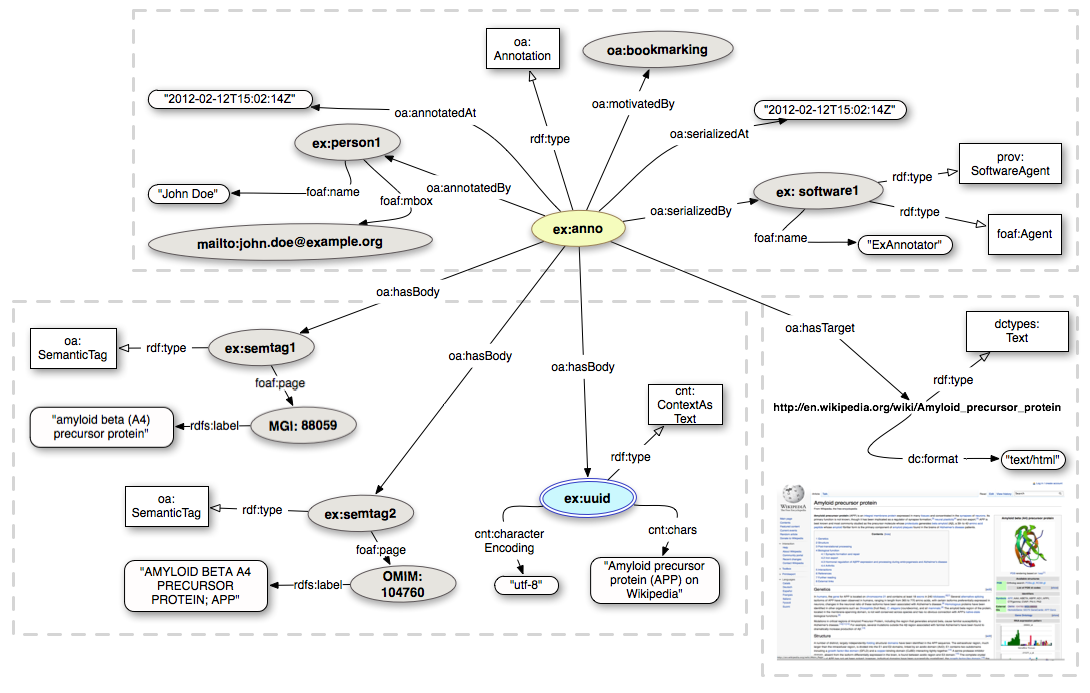
\includegraphics[width=1\linewidth]{Open-Annotation_CB_Bookmarking_and_Semantically_Tagging_A_webpage_spec20130128.png}
\end{adjustwidth}

\end{frame}

\begin{frame}
  \frametitle{Document authoring and storage}
  In most cases documents are created as a result of
  \begin{itemize}
  \item creative activity of a person with text processors (authoring);
  \item printing a digital copy or a data record in a database;
  \item aggregation operation over database records (report).
  \end{itemize}
  Then it is stored either as a physical paper and/or a digital document (PDF, DOCX, HTML).

  Since 2000-th, Semantic Web and Linked Open Data (LOD) is being developed, allowing
  \begin{itemize}
  \item structural storage of data within published documents;
  \item processing stored data computationally;
  \item integration of data structures and data objects globally.
  \end{itemize}

  The \textbf{aim of this research} is to develop technologies, software and services allowing construction of digital archives supporting document data inclusion and inference from existing documents.
\end{frame}

% \begin{frame}[fragile]
%   \frametitle{Representation}
%   % \begin{block}{}
%   %   \textbf{Целью} исследования является создание методики разработки процедур трансформации (PD\footnote{Platform [description] model.}) в виде ОО-модулей.
%   % \end{block}
%   % \begin{columns}
%   %   \begin{column}{0.5\linewidth}
%   %     % \includegraphics[width=1\linewidth]{pics/scenario-ru-wo-mothur.pdf}
%   %   \end{column}
%   %   \begin{column}{0.6\linewidth}
%   %     Задачи исследования:
%   %     \begin{itemize}
%   %     \item Изучить синтаксические структуры Logtalk в аспекте структурирования знаний;
%   %     \item Предложить методику представления трансформации в виде ОО-модулей;
%   %     \item Реализовать библиотеку объектов и классов для МДА;
%   %     \item Тестирование библиотеки на примере.
%   %     \end{itemize}
%   %   \end{column}
%   % \end{columns}

% \begin{adjustwidth}{-1.5em}{-1.5em}
% \begin{minted}[escapeinside=||,fontsize=\btprgsize]{xml}
% <html lang="ru" xmlns=http://www.w3.org/1999/xhtml
% |\GB{xmlns:taa}|=http://irnok.net/engine/rdfa-manipulation
% xml:lang="ru" metal:define-macro="page">
% <head> . . . . </head>
% <body prefix="rdf: http://www.w3.org/1999/...-ns# foaf: http://xmlns.com/foaf/...
% imei: imei.html# course: https://irnok.net/college/plan/01..16-...\
% %D0\%BA_PB-SM.plm.xml.xlsx-....2.3.1.html#"  resource="#post"
% typeof="schema:CreativeWork sioc:Post prov:Entity">
% <!-- The application control panel -->

% <main lang="ru" resource="#annotation" typeof="oa:Annotation" id="main-doc-cnt">
% <div property="oa:hasTarget" resource="#course-work-prog"></div>
% <article property="oa:hasBody" typeof="foaf:Document curr:WorkingProgram"
%          resource="#course-work-program" id="main-document">
%   <div |\GB{taa:content}|="imei:title-page"></div>
%   <div |\GB{taa:content}|="imei:neg-UMK"></div>
%   <section id="TOC" class="break-after"> <h2>Table of Contents</h2>
%     <div id="tableOfContents"></div>
%   </section>
%   <section id="course-description" resource="#description"
%            property="schema:hasPart" typeof="schema:CreativeWork">
%     <div property="schema:hasPart" resource="#purpose"
%          typeof="dc:Text cnt:ContentAsText" >
%       <div property="cnt:chars" datatype="xsd:string">
%         <h2 property="dc:title" datatype="xsd:string">
%            Aims and objectives of the discipline (module)</h2>
%         <p>The aim of teaching the discipline ...</p>
%       </div>
%    </div>
%   . . . . . . . .
% \end{minted}
% \end{adjustwidth}
% \end{frame}

% \begin{frame}
%   \frametitle{Linked Open Data, LOD}
%   \begin{enumerate}
%   \item Information is published in Internet with open access license;
%   \item It is represented in a machine-readable form, e.g., Excel table instead of a bitmap picture;
%   \item An open format used, e.g., CSV instead of Excel;
%   \item The format is based on W3C recommended standards, allowing RDF and SPARQL reference;
%   \item Published data refer to objects, forming context.
%   \end{enumerate}
%   Thus, applications publish data as relations of objects (entities).
% \end{frame}

\begin{frame}
  \frametitle{Logtalk as transformation definition language}
  We have chosen Logtalk as it
  \begin{itemize}
  \item inherits widely known Prolog language syntax and runtime
  \item implemented as macro package, performance penalties are about 1.5\%
  \item has flexible semantics: we can define transformations and constraints within the same syntax
  \item implement object-oriented knowledge (rules) structuring, encapsulation and replacement
  \item compositional way of transformation implementation
  \item powerful engine to post constraints on object-to-object messages (events)
  \item has implementation for many Prolog engines.
  \end{itemize}
  The <<regular>> language allow us to use its libraries not directly related to MDA transformations.
\end{frame}



\end{document}

%%% Local Variables:
%%% mode: latex
%%% TeX-master: t
%%% End:
